% ==============================================================
% Appendix for IKP Paper
% Auto-generated from evaluation data
% ==============================================================

\section{Probe Generation Methodology}
\label{app:probes}

This appendix expands Section~\ref{sec:probe-generation} with the full reproducibility detail of the IKP probe pipeline: tier definitions, per-corpus sampling procedures, quality filters with their drop rates, the final per-tier composition, verification procedure, and sample probes.

\subsection{Tier Definitions}
\label{app:tier-defs}

Each of the seven IKP tiers is defined by a calibrated parameter range: the model size at which a model with typical training-data coverage starts answering reliably. Tier targets are then \emph{validated} against the landmark ladder (Section~\ref{sec:tiers}); probes whose landmark behavior contradicts the assigned tier are reassigned or dropped.

\begin{table}[H]
\centering
\small
\setlength{\tabcolsep}{4pt}
\begin{tabularx}{\linewidth}{@{}l l l X@{}}
\toprule
\textbf{Tier} & \textbf{Name} & \textbf{Param range} & \textbf{Example} \\
\midrule
T1 & Universal Knowledge & 0.1B--0.5B & ``What is the capital of Norway?'' (Oslo) \\
T2 & Common Reference Knowledge & 0.5B--7B & ``Who composed the Enigma Variations?'' (Edward Elgar) \\
T3 & Domain-Specific Knowledge & 7B--32B & ``In what year was the Battle of Hastings fought?'' (1066) \\
T4 & Obscure Knowledge & 32B--235B & ``In computer science, what is the research subfield of Peter Druschel?'' (computer networking) \\
T5 & Deep Knowledge & 235B--1T & ``In what year was the town of Eliot in York County, Maine founded?'' (1810) \\
T6 & Long-Tail Knowledge & 1T--10T & ``In computer science, what is the research subfield of Jeffrey Helt?'' (distributed systems) \\
T7 & Extreme Long-Tail & $>$10T & ``In what country is the mountain Tadekho Hill located?'' (Canada) \\
\bottomrule
\end{tabularx}
\caption{Tier definitions used during probe generation. Parameter range is the model size at which a typically-trained model begins answering reliably; T7 is by construction beyond all current models and used as a ceiling probe. Examples here match those in Appendix~\ref{app:sample-probes}.}
\label{tab:tier-defs}
\end{table}

\subsection{Phase A: LLM-Generated Candidates}

Phase A targets T1--T2 saturation and supplementary fill at T3--T4. We use GPT-5 as the candidate generator with a structured prompt that:
(i)~specifies the target tier's parameter range and exemplar Q/A pairs,
(ii)~rotates a primary region (8 regions: North America, Europe, East Asia, South Asia, Middle East, Africa, Latin America, Oceania) and primary domain (6 domains: people, places, publications, measurements, events, organizations) per generation batch,
(iii)~requests 50 candidates per batch with $\geq 3$ paraphrases each, and
(iv)~requires verifiable, single-token-or-short-string gold answers.

\textbf{Yield.} 401 of 1{,}400 final probes ($28.6\%$) come from Phase A: T1 $n{=}166$, T2 $n{=}152$, T3 $n{=}51$, T4 $n{=}32$. The empirical tier distribution of LLM-generated candidates is heavily skewed toward T1--T2 (${\sim}82\%$) regardless of difficulty prompting, confirming that an LLM is structurally unable to generate probes beyond its own knowledge horizon---the central reason Phase B exists.

\subsection{Phase B: Corpus-Grounded Probes}

Phase B grounds probes in two external corpora whose ground-truth answers can be verified independently of any LLM.

\paragraph{Wikidata-grounded probes (557 probes).} We use Wikidata~\citep{vrandecic2014wikidata} SPARQL queries to sample entities from six categories: universities, journals, museums, bridges, sports clubs, and geographic places. Per-category SPARQL queries filter on entity type (P31 / instance of), require a published founding year (P571) or equivalent property, and stratify by Wikipedia article monthly-views-as-of-2025 to target a specific tier. Gold answers are read directly from the queried Wikidata property value. T3--T7 receive 94, 111, 100, 141, 100 Wikidata probes respectively.

\paragraph{Researcher subfield probes (345 probes).} Computer-science researchers are sampled from DBLP and OpenAlex, stratified by citation-count buckets (10--50 citations for T7, 50--500 for T6, 500--5{,}000 for T5, 5{,}000--50{,}000 for T3/T4). Each researcher's primary subfield is initially assigned from the dominant DBLP venue tag via a venue $\to$ subfield mapping table (e.g., SOSP/OSDI $\to$ ``operating systems''; SIGCOMM $\to$ ``computer networking''; CRYPTO $\to$ ``computer security''; SIGMOD/VLDB $\to$ ``database systems''; STOC/FOCS $\to$ ``theoretical computer science''). T5--T7 each receive 100, 59, 100 researcher probes; T3--T4 receive 35 and 51.

\textbf{Probe template.} The released format is two-part:
\begin{quote}
\itshape In computer science, what is the research subfield of \emph{Name}, and name one paper, system, institution, or co-author associated with their work? If you don't know who this person is, say so.
\end{quote}
The CS scoping (``In computer science'') reduces cross-field name collisions for short / common names. The artifact requirement (``name one paper, system, institution, or co-author'') is the load-bearing change: it forces models to produce a verifiable token that can be cross-checked against ground truth, rather than emitting a plausible-sounding but unattested CS subfield label. Without this requirement, a model that has never encountered ``Dan Schatzberg'' can still get full credit by guessing ``computer architecture'' (a popular subfield), since OpenAlex tags him as such; with the requirement, the model must additionally name TMO, EbbRT, ASPLOS, ISCA, Boston University, Meta, or some other token in his actual research footprint.

\textbf{Per-researcher evidence bundle.} Each researcher carries a structured gold record built from their OpenAlex profile and, for the tail of name-collision-flagged researchers, manually web-verified:
\begin{itemize}[leftmargin=*,topsep=2pt,itemsep=1pt]
    \item \texttt{primary\_subfield}: one of $\sim$17 CS subfield labels.
    \item \texttt{secondary\_subfields}: 0--3 acceptable adjacent labels for researchers whose work spans multiple subfields.
    \item \texttt{affiliations}: top 1--2 last-known institutions.
    \item \texttt{named\_systems}: short, capitalized system / artifact tokens extracted from paper titles by a regex pass over the top 10 most-cited works (e.g., ``TMO'', ``Zoltan'', ``Wukong'').
    \item \texttt{venues}: top 5--6 publication venues from the same set.
    \item \texttt{co\_authors}: top 5 collaborators ranked by joint-paper count.
    \item \texttt{top\_works}: top 5 paper titles with publication years and citation counts.
\end{itemize}

\textbf{Four-way evidence-aware judge.} Responses are classified into four classes, scored at $\lambda=-1$ for WRONG:
\begin{itemize}[leftmargin=*,topsep=2pt,itemsep=1pt]
    \item \textbf{CORRECT-STRONG} (score $+1.0$): response names \texttt{primary\_subfield} (or a direct synonym, or a listed \texttt{secondary\_subfield}) \emph{and} cites at least one matching evidence item---a system from \texttt{named\_systems}, a venue from \texttt{venues}, an affiliation from \texttt{affiliations}, a co-author from \texttt{co\_authors}, or a paper-title fragment overlapping with \texttt{top\_works}.
    \item \textbf{CORRECT-WEAK} (score $+0.5$): response names a primary or secondary subfield but cites no specific evidence (e.g., ``computer architecture, focusing on memory systems and cache coherence'' for a researcher with no actual cache work).
    \item \textbf{REFUSAL} (score $0$): response says ``I don't know'', expresses uncertainty, or declines.
    \item \textbf{WRONG} (score $\lambda=-1$): response names a CS subfield outside \{primary, secondary\} \emph{or} confidently fabricates specifics that contradict / are absent from the evidence bundle.
\end{itemize}
The score formula $\lambda \cdot \mathbb{1}[\text{WRONG}] + 0.5 \cdot \mathbb{1}[\text{WEAK}] + 1.0 \cdot \mathbb{1}[\text{STRONG}]$ makes confident bluffing strictly worse than refusing, while still rewarding partial knowledge (WEAK) above refusal.

\textbf{Name-collision sub-class.} Sixteen names (all in T7) had no real CS researcher despite OpenAlex listing a person under that name (the OpenAlex profile pointed at, e.g., a chemist, virologist, or radiologist with the same name). These were replaced with web-verified CS researchers in the same subfield, re-calibrated through the 6-landmark ladder, and re-confirmed as T7 (no landmark answers correctly).

\paragraph{Manual / supplementary probes (97 probes).} A small set of high-quality probes were manually authored or carried over from earlier dataset versions to balance per-tier coverage in T1--T4 where automated sampling was insufficient.

\subsection{Quality Filters and Drop Rates}

Four filters are applied to every candidate before inclusion. Each filter is conservative (false positives drop legitimate probes; false negatives admit problematic ones, which we accept as long as the rate is bounded):

\begin{enumerate}[leftmargin=*,topsep=2pt,itemsep=1pt]
    \item \textbf{Computable knowledge filter.} Drops probes whose answer can be derived by rule rather than memorization: arithmetic on years (``what year was X 10 years ago''), alphabetical/ordinal answers, IUPAC chemical naming, etc. Implementation: regex + LLM classification, manual review of edge cases.
    \item \textbf{Monotonicity filter.} A probe is admitted only if accuracy across the landmark ladder (Section~\ref{sec:tiers}) is monotonic non-decreasing in landmark capability. Probes where a smaller landmark answers correctly while a larger one does not---typically caused by ambiguous phrasing, multi-valued ground truth, or judge errors---are dropped. Drops $\sim 15\%$ of post-Phase-B candidates.
    \item \textbf{Name-collision filter (researcher probes).} Drops two-character Chinese names and single-initial given names where multiple distinct researchers share the identifier; a 50-citation Liu Yang and a 5{,}000-citation Liu Yang are not the same person. Implementation: cross-check unique \emph{(name, affiliation)} tuples against DBLP author IDs.
    \item \textbf{Contamination filter (researcher probes).} Drops researchers in machine-learning, deep-learning, NLP, computer vision, and reinforcement-learning subfields. These authors' own work disproportionately appears in frontier-model training corpora, inflating accuracy in a way that conflates IKP-style long-tail knowledge with training-set memorization of one's own field. The remaining 14 CS subfields (systems, databases, security, networking, theory, etc.) are kept.
    \item \textbf{Question-template grounding filter.} For Wikidata-sourced probes, every question template embeds a discriminating attribute---year, country, administrative region, genre, language, or publisher---extracted from a Wikidata field that is \emph{not} the answer field. This is the same design used by researcher probes (which prefix every question with ``In computer science''). The filter exists because an audit of the bare-name templates (``In what year was X founded?'') revealed silent failures under title collision: ``Putnam'' could refer to Putnam, Connecticut (Wikidata's intended entity) or Putnam County, Florida; ``Madonna and Child'' refers to dozens of Renaissance paintings. Grounding raises the within-probe identifiability bar without leaking the answer (e.g., ``Who painted the 1522 painting `The Virgin of Carmel'?'' grounds via year without naming the artist). The grounded template is generated programmatically from Wikidata claims at SPARQL time, then independently re-calibrated through the landmark ladder---a non-trivial post-condition, since grounding tends to make probes easier and shift them out of T6/T7. In our audit, $\sim 30\%$ of grounded T7 candidates re-calibrated to T5 (became too easy with grounding) and ${\sim}5\%$ became non-monotonic; the surviving $\sim 65\%$ form the released T6/T7 Wikidata pool.
\end{enumerate}

\subsection{Final Composition}
\label{app:probe-composition}

\begin{table}[H]
\centering
\small
\begin{tabular}{l rrrrr}
\toprule
\textbf{Tier} & \textbf{LLM} & \textbf{Wikidata} & \textbf{Researcher} & \textbf{Manual} & \textbf{Total} \\
\midrule
T1 & 166 & 6   & 0   & 28 & 200 \\
T2 & 152 & 5   & 0   & 43 & 200 \\
T3 & 51  & 94  & 35  & 20 & 200 \\
T4 & 32  & 111 & 51  & 6  & 200 \\
T5 & 0   & 100 & 100 & 0  & 200 \\
T6 & 0   & 141 & 59  & 0  & 200 \\
T7 & 0   & 100 & 100 & 0  & 200 \\
\midrule
\textbf{Total} & 401 & 557 & 345 & 97 & \textbf{1{,}400} \\
\bottomrule
\end{tabular}
\caption{Per-tier probe composition by source. ``Manual'' aggregates manually-authored and supplementary probes from earlier dataset iterations. The dominance of researcher and Wikidata probes at T5--T7 reflects the unavoidability of corpus grounding at frontier difficulty.}
\label{tab:probe-composition}
\end{table}

For T5--T7 specifically, the dominant domain is computer-science researcher subfield (259/600 probes, $43\%$). The remaining T5--T7 Wikidata probes span 16 fact types after the audit (Section~\ref{sec:wikidata-audit}): grounded founding years (sports clubs, museums, bridges, universities, journals, abbeys, tramways), and entity-attribute questions (river mouths, film directors, capes, sculptors, founders, mountains, lakes, painters, screenwriters, composers, named-after eponyms, headquarters cities, architects). The original T6/T7 Wikidata composition was a 100\% founding-year monoculture; the audit replaced ${\sim}50\%$ of T6/T7 Wikidata probes with diverse fact types to remove that source bias while preserving the unambiguous-answer property.

\subsection{Verification Procedure}

Gold-answer verification differs by source:

\begin{itemize}[leftmargin=*,topsep=2pt,itemsep=2pt]
    \item \textbf{Wikidata probes}: gold answer is the queried property value as of the SPARQL extraction date. Conflicts (e.g., a museum with multiple founding-date claims) are resolved by selecting the value with the most reference citations; probes with unresolved conflicts are dropped. After an audit (Section~\ref{sec:wikidata-audit}), every T5--T7 Wikidata probe was independently web-cross-checked against Wikipedia and primary sources; probes with a Wikidata-vs-Wikipedia disagreement on the answer were either corrected (4 cases, e.g.\ Makran Medical College: Wikidata 2015, Wikipedia 2017---kept Wikipedia's answer) or dropped (e.g., probes attributing a sculpture to its bronze foundry rather than its sculptor). All probes whose answers were corrected were re-calibrated through the landmark ladder, since changing the gold answer changes which landmarks are scored as correct and therefore the assigned tier.
    \item \textbf{Researcher probes}: gold subfield is derived from each researcher's dominant DBLP venue tag in their highest-cited 5 papers, mapped to one of 14 CS subfields. Researchers whose top-5 papers split across $\geq 3$ unrelated subfields are dropped (only researchers with a clear primary specialization are retained).
    \item \textbf{Phase A probes}: gold answers are produced by the generator and independently re-verified by a different LLM (Claude Opus 4.6) plus a manual spot-check of $\sim 10\%$.
    \item \textbf{Manual probes}: directly authored with citation evidence.
\end{itemize}

\subsection{Sample Probes}
\label{app:sample-probes}

\begin{table}[htbp]
\centering
\small
\setlength{\tabcolsep}{4pt}
\renewcommand{\arraystretch}{1.15}
\begin{tabular}{@{}c l p{0.55\linewidth} l@{}}
\toprule
\textbf{Tier} & \textbf{Source} & \textbf{Question} & \textbf{Answer} \\
\midrule
\multirow{3}{*}{T1} & Wikidata   & What is the capital of Norway? & Oslo \\
                    & LLM        & In what year was the Meiji Constitution promulgated? & 1889 \\
                    & LLM        & Who designed the Sydney Opera House? & Jørn Utzon \\
\midrule
\multirow{3}{*}{T2} & LLM        & Who composed the Enigma Variations? & Edward Elgar \\
                    & LLM        & What is the most common isotope of hydrogen? & Protium \\
                    & Manual     & Who was the first Prime Minister of India? & Jawaharlal Nehru \\
\midrule
\multirow{3}{*}{T3} & LLM        & In what year was the Battle of Hastings fought? & 1066 \\
                    & Wikidata   & In what year was Hunan Normal University founded? & 1938 \\
                    & Manual     & What year was the Camp David Accords signed? & 1978 \\
\midrule
\multirow{3}{*}{T4} & Researcher & In computer science, what is the research subfield of Peter Druschel, and name one paper, system, institution, or co-author associated with their work? If you don't know who this person is, say so. & computer networking \\
                    & Wikidata   & In what year was Lawrence Heritage State Park founded? & 1980 \\
                    & Wikidata   & In what year was the journal \textit{Cancer} first published? & 1948 \\
\midrule
\multirow{3}{*}{T5} & Wikidata   & In what year was the town of Eliot in York County, Maine founded? & 1810 \\
                    & Researcher & In computer science, what is the research subfield of Jianliang Xu, and name one paper, system, institution, or co-author associated with their work? If you don't know who this person is, say so. & data mining \\
                    & Wikidata   & In what year was State Polytechnic of Indramayu founded? & 2014 \\
\midrule
\multirow{3}{*}{T6} & Researcher & In computer science, what is the research subfield of Jeffrey Helt, and name one paper, system, institution, or co-author associated with their work? If you don't know who this person is, say so. & distributed systems \\
                    & Wikidata   & In what year was Museu da Misericórdia founded? & 2006 \\
                    & Wikidata   & In what year was Universitas Imelda Medan founded? & 2019 \\
\midrule
\multirow{3}{*}{T7} & Wikidata   & In what country is the mountain Tadekho Hill located? & Canada \\
                    & Researcher & In computer science, what is the research subfield of Christopher Bengel, and name one paper, system, institution, or co-author associated with their work? If you don't know who this person is, say so. & computer architecture \\
                    & Wikidata   & Into what body of water does the Bolshaya Khopa in Arkhangelsk Oblast, Russia flow? & Soyana \\
\bottomrule
\end{tabular}
\caption{Three sample probes per tier, one per source where possible. Each row is a single probe as it appears in the released probe set.}
\label{tab:sample-probes}
\end{table}

Table~\ref{tab:sample-probes} lists three representative probes per tier, drawing from all three probe sources (LLM-generated, Wikidata-grounded, researcher subfield) so that each contributes.

\section{Hallucination Penalty Sensitivity}
\label{app:lambda}

The hallucination penalty $\lambda$ (a wrong answer scores $\lambda$; correct $=+1$, refusal $=0$) is a scoring-convention choice. This appendix reports its sensitivity: it sweeps $\lambda$ over $\{0,\,-0.25,\,-0.5,\,-1.0,\,-2.0\}$, refits the log-linear calibration on the same 93-model open-weight set for each value, and re-inverts for four flagship proprietary models (Table~\ref{tab:lambda-sweep}). The released dataset, companion website, and estimation toolkit (\texttt{scripts/ikp\_estimate.py}) default to $\lambda = 0$ (raw accuracy), so that IKP accuracy is directly the fraction of probed facts a model answers correctly with no scoring convention to interpret; the table lets results under any penalty be read off directly.

\begin{table}[H]
\centering
\small
\caption{Sensitivity of the IKP calibration and of four flagship proprietary estimates to the hallucination penalty $\lambda$. Each row refits $A = \alpha \log_{10}(N) + \beta$ on the same 93 open-weight models, recomputing every model's accuracy from stored verdicts under the listed $\lambda$ (correct $=+1$, refusal $=0$, wrong $=\lambda$), and re-inverts the fit for each flagship model. ``Slope'' is in percentage points per decade; ``LOO$\times$'' is the median multiplicative parameter-prediction error in leave-one-out cross-validation; ``PI$\times$'' is the 90\% prediction-interval factor. $\lambda = 0$ (starred) is the default used by the released dataset, website, and toolkit. Table generated by \texttt{scripts/lambda\_sensitivity.py}.}
\label{tab:lambda-sweep}
{\setlength{\tabcolsep}{4pt}\begin{tabular}{rccccrrrr}
\toprule
$\lambda$ & Slope & $R^2$ & LOO$\times$ & PI$\times$ & GPT-5.5 Pro & Claude Fable 5 & GPT-4.1 & Claude Opus 4.7 \\
 & (pp/dec) & & (med.) & (90\%) & est. & est. & est. & est. \\
\midrule
$0.00$\;$^\star$ & 15.9 & 0.910 & 1.48 & 3.20 & 5.3T & 3.5T & 2.2T & 538B \\
$-0.25$ & 16.7 & 0.936 & 1.48 & 2.64 & 4.6T & 4.3T & 1.6T & 761B \\
$-0.50$ & 16.6 & 0.935 & 1.57 & 2.65 & 5.2T & 4.9T & 1.5T & 916B \\
$-1.00$ & 16.5 & 0.934 & 1.65 & 2.68 & 5.7T & 4.8T & 1.2T & 1.2T \\
$-2.00$ & 16.0 & 0.920 & 1.68 & 2.99 & 5.4T & 5.8T & 1.3T & 1.5T \\
\bottomrule
\end{tabular}
}
\end{table}

\textbf{Findings.} (i)~Fit quality is near-flat across the band: $R^2$ ranges only ${\sim}0.90$--$0.93$ and the 90\% PI factor ${\sim}2.7$--$3.5\times$, so the calibration is robust to the penalty choice. (ii)~We adopt $\lambda = 0$ (raw accuracy) as the operating point for \emph{interpretability}: with no penalty, IKP accuracy is directly the fraction of probed facts a model answers correctly, requiring no scoring convention to read. This costs ${\sim}0.02$--$0.03$ in $R^2$ relative to the shallow optimum near $\lambda = -0.5$ and slightly widens the prediction interval---a tradeoff we accept in exchange for a directly-meaningful accuracy metric. (iii)~Individual estimates shift with $\lambda$ in a \emph{vendor-dependent} way (last four columns of Table~\ref{tab:lambda-sweep}): a heavier penalty raises the estimates of models that refuse rather than bluff (e.g.\ Claude Opus~4.7, $0.55 \to 1.5$T from $\lambda = 0$ to $-2$) and lowers those of confident guessers (e.g.\ GPT-4.1, $2.2 \to 1.1$T), because it reattributes above-trend scores from confident hallucination to genuine capacity. Readers who prefer a hallucination-aware metric can read any column of Table~\ref{tab:lambda-sweep} directly; the qualitative frontier ordering is preserved within each column.

\begin{figure}[H]
\centering
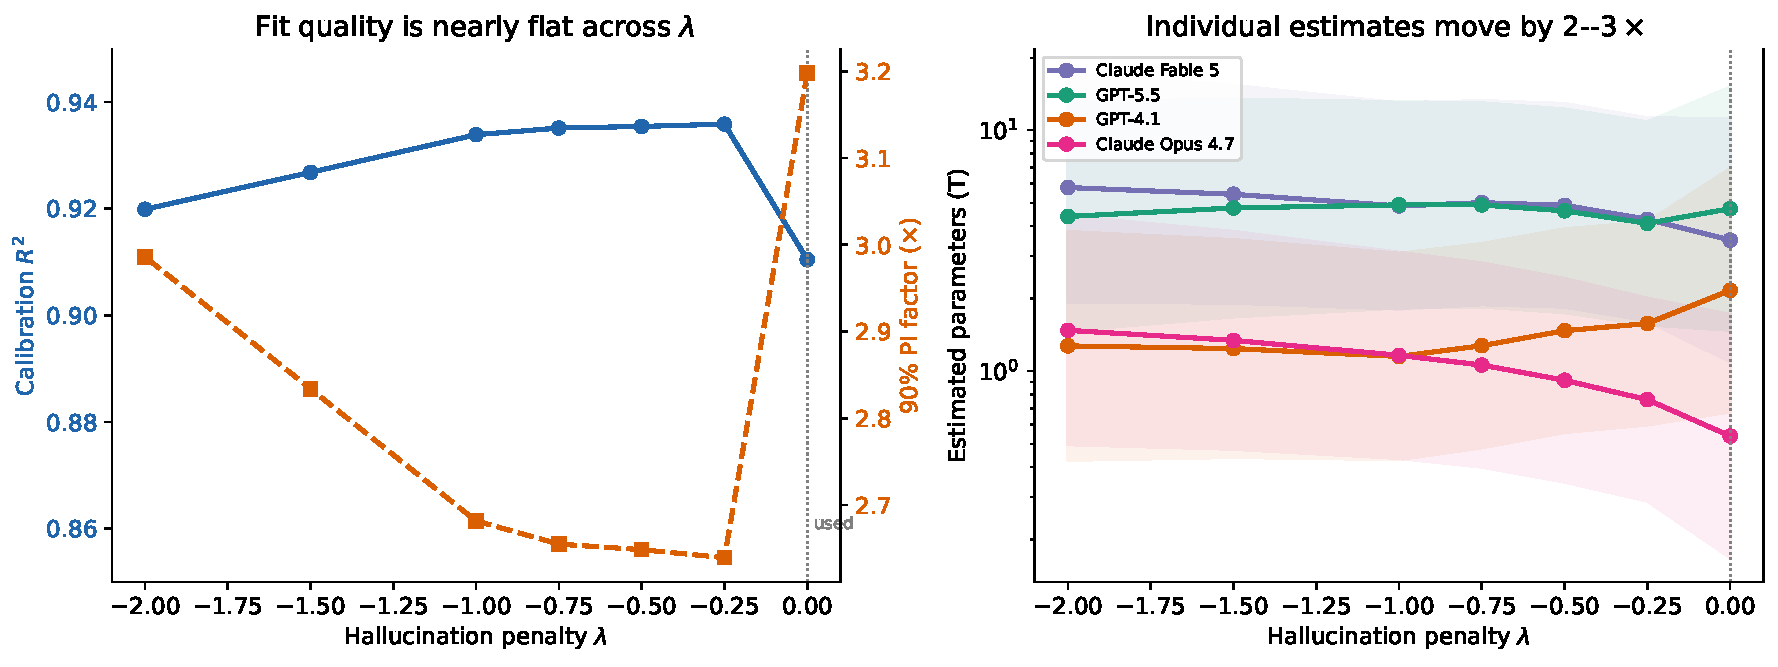
\includegraphics[width=\textwidth]{figures/fig_lambda_sensitivity.pdf}
\caption{What changes across the hallucination penalty $\lambda$. \textbf{Left:} calibration fit quality is nearly flat---$R^2$ stays in $[0.91,0.94]$ and the 90\% prediction-interval factor in $[2.6,3.2]\times$ (floored scoring for $\lambda<0$; $\lambda=0$ is floor-free). \textbf{Right:} individual frontier estimates (90\% bands shaded) move by $2$--$3\times$ and \emph{re-order} by vendor: as $\lambda\to 0$ the confident guesser GPT-4.1 rises while the refusal-heavy Claude Opus~4.7 falls. Generated by \texttt{scripts/../paper/figures/generate\_lambda\_figure.py}.}
\label{fig:lambda}
\end{figure}

\textbf{The $\lambda$-choice principle.} We fix $\lambda$ by \emph{parsimony}, not by tuning. The rule is: adopt the parameter-free operating point---$\lambda = 0$, which simultaneously eliminates the flooring rule (per-tier scores are then $\geq 0$ by construction)---\emph{unless} a nonzero penalty materially improves the calibration. It does not: across $\lambda \in [0, -2]$ the calibration $R^2$ varies by ${\leq}0.03$ and the 90\% PI factor by ${\leq}0.6\times$ (Figure~\ref{fig:lambda}, left), and the frontier ordering is preserved within each column (Table~\ref{tab:lambda-sweep}). A nonzero $\lambda$ therefore buys at most $0.03$ in $R^2$ at the price of \emph{two} tunable knobs---the penalty magnitude and the floor---that, as Table~\ref{tab:floor-ablation} shows, can together be dialed to inflate frontier estimates by $3$--$5\times$. Because IKP is a measurement instrument, we prefer the estimator a reader cannot tune toward a desired answer, and $\lambda = 0$ is that Schelling point. This is a principled default, not a convenience: readers who prefer a hallucination-aware score may read any $\lambda$ column directly, accepting the $2$--$3\times$ vendor-dependent shift of Figure~\ref{fig:lambda} (right)---but no qualitative conclusion of the paper depends on the choice.

\subsection{Flooring and its interaction with $\lambda$}
\label{app:flooring}

A second scoring degree of freedom is whether per-tier scores are floored at zero. Under a negative penalty a strongly-bluffing model can score negative on the hard tiers; flooring those scores at zero raises small/aggressive models' accuracy, which flattens the calibration slope and---because the curve is inverted to estimate size---inflates frontier estimates. Table~\ref{tab:floor-ablation} crosses $\lambda$ with flooring on/off.

\begin{table}[H]
\centering
\small
\caption{Calibration and two flagship estimates under $\lambda \times$ flooring. Flooring only matters under a negative penalty; unfloored, the fit degrades sharply as $|\lambda|$ grows ($R^2$ from $0.91$ to $0.72$, PI factor from $3.2\times$ to $9.9\times$) because negative hard-tier scores dominate the regression, and estimates fall by up to ${\sim}3\times$. At $\lambda = 0$ (starred) the floor is a no-op, so the ambiguity vanishes entirely---the principal reason we adopt no-penalty scoring. Generated by \texttt{scripts/lambda\_floor\_ablation.py}.}
\label{tab:floor-ablation}
{\setlength{\tabcolsep}{5pt}\begin{tabular}{rlrrrrrr}
\toprule
$\lambda$ & floor & $R^2$ & Slope & PI$\times$ & LOO$\times$ & GPT-5.5 & Gemini 3.1 Pro \\
 & & & (pp/dec) & & & est. & est. \\
\midrule
$0.00$$^\star$ & on & 0.910 & 15.9 & 3.20 & 1.48 & 4.7T & 7.3T \\
\multicolumn{8}{l}{\footnotesize\quad(at $\lambda=0$ the floor is a no-op: scores are $\text{correct}/\text{total}\geq 0$)} \\
$0.00$ & off & 0.910 & 15.9 & 3.20 & 1.48 & 4.7T & 7.3T \\
$-0.25$ & on & 0.936 & 16.7 & 2.64 & 1.48 & 4.1T & 9.4T \\
$-0.25$ & off & 0.931 & 19.3 & 2.74 & 1.56 & 3.0T & 6.2T \\
$-0.50$ & on & 0.935 & 16.6 & 2.65 & 1.57 & 4.6T & 12.0T \\
$-0.50$ & off & 0.905 & 22.7 & 3.32 & 1.55 & 2.2T & 5.5T \\
$-1.00$ & on & 0.934 & 16.5 & 2.68 & 1.65 & 4.9T & 18.0T \\
$-1.00$ & off & 0.830 & 29.5 & 5.35 & 1.77 & 1.5T & 4.8T \\
$-1.50$ & on & 0.927 & 16.3 & 2.83 & 1.63 & 4.8T & 25.4T \\
$-1.50$ & off & 0.768 & 36.4 & 7.66 & 2.12 & 1.2T & 4.3T \\
$-2.00$ & on & 0.920 & 16.0 & 2.99 & 1.68 & 4.4T & 34.5T \\
$-2.00$ & off & 0.723 & 43.2 & 9.91 & 2.40 & 972B & 4.1T \\
\bottomrule
\end{tabular}
}
\end{table}

\textbf{Relation to prior discrepancy.} An earlier version of IKP reported floored scores under $\lambda = -1.0$ while the accompanying text described the scores as unfloored; the two differ materially (e.g.\ GPT-5.5 $4.9$T floored vs.\ $1.5$T unfloored at $\lambda=-1.0$). Adopting $\lambda = 0$ removes the discrepancy at its root: with no penalty every per-tier score is $\text{correct}/\text{total} \geq 0$, so floored and unfloored scoring are identical and there is nothing left to specify.

\section{Dense vs.\ MoE Calibration}
\label{app:moe}

The calibration pools dense and Mixture-of-Experts models; Table~\ref{tab:moe-fits} fits them separately. The per-decade slope is nearly identical (dense $0.151$, MoE-total $0.145$), but MoE-total sits slightly higher---an MoE knows ${\sim}2$--$4$ pp more per \emph{total} parameter than a same-size dense model---and fits more loosely ($R^2=0.67$ vs $0.88$). Active parameters predict MoE knowledge far worse ($R^2=0.41$), confirming that factual capacity scales with \emph{total}, not active, weights: an MoE with $T$ total and $A$ active parameters behaves, for recall, like a dense model of ${\sim}T$ parameters. Notably the combined-set slope ($0.159$) is \emph{steeper} than either subset---a mixture effect, since MoE models cluster at large $N$/high accuracy and dense at small $N$/low accuracy.

\begin{table}[H]
\centering\small
\caption{Log-linear calibration fit by architecture ($\lambda=0$, cleaned set). Generated by \texttt{scripts/moe\_dense\_analysis.py}.}
\label{tab:moe-fits}
\begin{tabular}{lrrrr}
\toprule
Calibration subset & $n$ & Slope & Intercept & $R^2$ \\
\midrule
Dense & 52 & 0.151 & 0.245 & 0.875 \\
MoE (total params) & 41 & 0.145 & 0.282 & 0.667 \\
MoE (active params) & 41 & 0.144 & 0.453 & 0.412 \\
Combined (headline) & 93 & 0.159 & 0.242 & 0.910 \\
\bottomrule
\end{tabular}

\end{table}

\textbf{Which curve should estimate (MoE) frontier models?} Frontier proprietary models are widely believed to be MoE, so one might fit only on MoE anchors. Empirically this does \emph{not} help. In leave-one-out over the 41 known-size open MoE models, the MoE-only curve recovers their sizes no better than the combined curve (median fold error $1.58\times$ vs.\ $1.52\times$ overall; $1.55\times$ vs.\ $1.55\times$ for the 34 models ${\geq}100$B). Dropping the 52 dense anchors to erase a ${\sim}2$--$4$ pp offset costs more in slope stability than the offset is worth, and per-model deviations from post-training, distillation, and refusal behavior---GLM over-knowing for its size by ${\sim}3\times$, DeepSeek V4 Pro's degraded non-thinking variant ${\sim}10\times$ low---dwarf the architecture gap. We therefore keep the combined curve as the headline: it is the \emph{validated} choice, not merely a convenient one.

\textbf{MoE-deflation caveat.} Because the combined slope is steeper, it assigns \emph{lower} sizes to the highest-accuracy models than a pure MoE curve would (Table~\ref{tab:moe-sens}): switching to the MoE-total curve raises the top estimates by ${\sim}18\%$ (e.g.\ Claude Fable 5 from ${\sim}3.5$T to ${\sim}4.0$T; GPT-5.5 from ${\sim}4.7$T to ${\sim}5.5$T). These shifts are well within the $3.2\times$ prediction interval and cannot be validated out-of-sample, so we report combined-curve values as headline while noting that presumed-MoE frontier models may be modestly under-placed.

\begin{table}[H]
\centering\small
\caption{Frontier estimate sensitivity to the calibration subset: headline combined curve vs.\ the MoE-total curve. Generated by \texttt{scripts/moe\_dense\_analysis.py}.}
\label{tab:moe-sens}
\begin{tabular}{lrrr}
\toprule
Model & Accuracy & Combined & MoE-curve \\
\midrule
Claude Fable 5 & 80.5\% & ${\sim}3.5$T & ${\sim}4.0$T \\
GPT-5.5 Pro & 83.4\% & ${\sim}5.3$T & ${\sim}6.3$T \\
GPT-5.5 & 82.6\% & ${\sim}4.7$T & ${\sim}5.5$T \\
Gemini 2.5 Pro & 79.5\% & ${\sim}3.0$T & ${\sim}3.4$T \\
GPT-4.1 & 77.2\% & ${\sim}2.2$T & ${\sim}2.4$T \\
Claude Opus 4.7 & 67.6\% & ${\sim}538$B & ${\sim}515$B \\
\bottomrule
\end{tabular}

\end{table}

\section{Wikidata Long-Tail Audit}
\label{app:wikidata-audit}

This appendix expands Section~\ref{sec:wikidata-audit}: it documents the failure-mode taxonomy uncovered when auditing the T5--T7 Wikidata-sourced probes against Wikipedia and primary sources, the per-round telemetry of the 10-round repair cycle, and the empirical observation that an answer-field correction necessarily invalidates the probe's prior tier assignment.

\subsection{Failure-Mode Taxonomy}

Every problematic probe falls into exactly one of five buckets. The taxonomy is intended to be a re-usable diagnostic for any future Wikidata-sourced evaluation set.

\begin{description}[leftmargin=2em,topsep=2pt,itemsep=2pt,style=nextline]
    \item[A. Wikidata-itself-wrong.] Outright incorrect facts in Wikidata that are falsifiable via Wikipedia or a primary source.
    \begin{itemize}[leftmargin=*,topsep=1pt,itemsep=1pt]
        \item \textbf{A1. Stale data} (\texttt{P159} headquarters typically): Roku still listed as headquartered in Los Gatos despite a 2019 move to San Jose; Vista Outdoor in Clearfield despite a move to Anoka. Frequency: $\sim 75\%$ of headquarters probes were stale.
        \item \textbf{A2. Wrong field semantics}: \texttt{P170} (creator) for sculptures often returns the bronze foundry, not the sculptor---Giacometti's \emph{L'Homme qui marche I} attributed to Susse Fr\`{e}res; Bourdelle's \emph{Monument to Alvear} attributed to Eug\`{e}ne Rudier.
        \item \textbf{A3. Self-referential / circular}: ``Na Klang named after Na Klang''---a Thai descriptive place-name (``middle field'') incorrectly marked as having an eponymous referent.
        \item \textbf{A4. Plain wrong year/value}: Makran Medical College listed as 2015 when Wikipedia infobox says 2017; Lady Snowblood screenplay attributed to the manga illustrator Kazuo Kamimura rather than the actual screenwriter Norio Osada.
    \end{itemize}
    \item[B. Pipeline extraction bugs (on our side).] \texttt{P571} inception was correct in Wikidata, but our SPARQL pipeline extracted a different date field (e.g., the year the building was constructed rather than the year the museum was chartered: George Eastman Museum stored as 1905, but Wikidata \texttt{P571}=1947).
    \item[C. Probe-construction ambiguity (Wikidata correct, question unanswerable).] The most prevalent class.
    \begin{itemize}[leftmargin=*,topsep=1pt,itemsep=1pt]
        \item \textbf{C1. Generic religious-art title}: ``Madonna and Child'', ``Holy Trinity'', ``Saint Apollonia''---each refers to dozens of works by different painters across centuries.
        \item \textbf{C2. Generic geographic-feature name}: ``Stone Bridge'' (Latvia? Russia? UK?), ``South Island'' (New Zealand? or the one in Lake Turkana, Kenya?), ``Hog Island'' (Falklands, or one of several US ones?), ``Devil's Lake''.
        \item \textbf{C3. Bare common-name place}: ``Putnam'' (the Connecticut town, or Putnam County?), ``Norwich'' (Vermont? or the much more famous Norwich, England?), ``Wells''.
        \item \textbf{C4. Generic institution name}: ``Maritime Museum'' (Jakarta? San Diego? Greenwich?), ``St. Lawrence University'' (Kampala, Uganda? or the famous one in NY?).
    \end{itemize}
    \item[D. Politically/legally contested entities.] Wikidata picks one answer where reasonable models will give a different one.
    \begin{itemize}[leftmargin=*,topsep=1pt,itemsep=1pt]
        \item \textbf{D1. Disputed sovereignty}: Loaita Cay listed under Vietnam (the cay is one of the Spratlys; claimed by China, Vietnam, and the Philippines). Cape Plaka listed under Ukraine (in Crimea, internationally recognized as Ukraine but Russian-occupied since 2014).
        \item \textbf{D2. Historical-vs-current statehood}: Mount Ashley listed under ``United Kingdom''---technically the South Georgia archipelago is its own British Overseas Territory, not part of the UK proper.
    \end{itemize}
    \item[E. Multi-actor attribution.] A genuinely correct attribution that is one of several equally valid answers; reasonable models will give a different one.
    \begin{itemize}[leftmargin=*,topsep=1pt,itemsep=1pt]
        \item \textbf{E1. Co-founder selection}: Cin\'{e}math\`{e}que de Tanger has 3 founders (Lahlou, Auriol, Barrada); the National Council of Women of Canada has Adelaide Hoodless (treasurer at founding) and Lady Aberdeen (first president).
        \item \textbf{E2. Co-author / story-vs-screenplay}: Twenty-Four Eyes screenplay attributed to the novelist Sakae Tsuboi rather than the actual screenwriter (and director) Keisuke Kinoshita; The Amazing Panda Adventure screenplay attributed to John Wilcox (story credit) rather than Jeff Rothberg / Laurice Elehwany (actual screenplay).
    \end{itemize}
\end{description}

The audit response by class: A and B are resolved by correcting the answer field (and re-calibrating); C is resolved by adding a discriminating qualifier to the question template (``the town of Putnam in Connecticut''); D is resolved by either dropping the probe (Loaita Cay) or accepting Wikidata's choice with the caveat that the LLM judge accepts the documented answer; E is resolved by accepting any of the multiply-valid answers via the judge's instruction to credit co-contributors.

\subsection{Per-Round Sourcing Telemetry}

Replacement probes were sourced via 10 SPARQL rounds, each producing 100--300 candidates that were calibrated through the landmark ladder. Per-fact-type web-verification pass rates emerged empirically and informed which fact types to over-source in later rounds.

\begin{table}[H]
\centering
\small
\setlength{\tabcolsep}{4pt}
\begin{tabularx}{\textwidth}{@{}>{\raggedright\arraybackslash}X r r l >{\raggedright\arraybackslash}X@{}}
\toprule
\textbf{Round} & \textbf{Sourced} & \textbf{Calib.\ valid} & \textbf{T6/T7 yield} & \textbf{Web-verified pass} \\
\midrule
R1 (founding-year)               & 186 & 155 & 70 (T6=25, T7=45) & --- (most rejected post-mandate) \\
R2 (mixed)                       & 152 & 138 & 39 (T6=20, T7=19) & 18/27 diverse (67\%) \\
R3 (composer/birthplace)         & 0   & --- & ---               & --- (SPARQL timeouts) \\
R4 (diverse-only)                & 140 & 124 & 24 (T6=10, T7=14) & 15/24 (62\%) \\
R5 (12 fact types)               & 250 & 228 & 68 (T6=39, T7=29) & 21/29 T7 (72\%) \\
R6 (11 fact types + castle)      & 275 & 256 & 64 (T6=36, T7=28) & 18/28 T7 (64\%) \\
R7 (7 reliable types only)       & 140 & 130 & 21 (T6=9, T7=12)  & 11/12 T7 (\textbf{92\%}) \\
R8 (aggressive ambiguity filter) & 100 & 92  & 24 (T6=13, T7=11) & 7/11 T7 (64\%) \\
R9 (most reliable types)         & 75  & 71  & 26 (T6=8, T7=18)  & 18/18 T7 (\textbf{100\%}) \\
R10 (grounded SPARQL templates)  & 45  & 15  & 5 (T6=3, T7=2)    & --- (low yield; alt path used) \\
\bottomrule
\end{tabularx}
\caption{Per-round sourcing telemetry. Total API spend across all rounds: ${\sim}10{,}000$ landmark+judge calls and ${\sim}120$ manual web verifications.}
\label{tab:audit-telemetry}
\end{table}

\subsection{Per-Fact-Type Reliability Ranking}

Aggregating across rounds 4--7, the empirical reliability of each Wikidata fact type at the long tail (T6/T7 obscurity):

\begin{enumerate}[leftmargin=*,topsep=2pt,itemsep=1pt]
    \item \textbf{\texttt{P403} river mouth} --- 100\% pass rate. Geography is well-curated.
    \item \textbf{\texttt{P57} director (film)} --- 67--100\% on attribution; ambiguity from generic film titles (``Night Train'', ``Hit Man'') is the dominant failure mode and is resolved by adding year + country + genre to the template.
    \item \textbf{\texttt{P17} country (cape/island/lake/mountain)} --- 75--100\%. Caveat: politically contested entities (Crimea, Spratlys, South Georgia) consistently fail web cross-check because Wikidata picks one claimant.
    \item \textbf{\texttt{P571} inception (founding year)} --- ${\sim}95\%$. The most-curated date field. Most failures trace to pipeline-side date-field selection bugs (Bucket B), not Wikidata error.
    \item \textbf{\texttt{P112} founder (organization)} --- 75\%. Sometimes returns the founding \emph{organization} rather than a person (e.g., St John Clinic founded by ``Order of the Holy Ghost''), making the question awkward when phrased ``Who founded \ldots?''.
    \item \textbf{\texttt{P170} creator (sculpture)} --- ${\sim}70\%$. The major Bucket-A2 failure: Wikidata's creator field for sculptures frequently records the bronze foundry rather than the sculptor.
    \item \textbf{\texttt{P58} screenwriter} --- 50\%. Routinely conflates ``story by'' credit with ``screenplay by'' credit (e.g., the manga author of \emph{Lady Snowblood} listed as the film's screenwriter).
    \item \textbf{\texttt{P159} headquarters} --- 25\%. \emph{Stale}. Wikidata frequently reflects a company's HQ from years prior; modern moves are not propagated quickly.
    \item \textbf{\texttt{P170} creator (painting)} --- ${\sim}70\%$ on attribution, but ${\sim}100\%$ title-collision rate at T6/T7 obscurity (generic religious-art titles). Painter probes are essentially unusable for T7 obscurity.
    \item \textbf{\texttt{P138} named after} --- mixed; self-referential and descriptive-placename errors observed.
\end{enumerate}

\section{Full Model Results}
\label{app:full-results}

Tables~\ref{tab:full-accuracy} and~\ref{tab:full-hallucination} present the complete evaluation results for all 188 models.
Models are grouped by vendor and sorted by overall penalized accuracy (descending) within each group.
Vendors are ordered by the highest accuracy achieved by any model in that group.
The \emph{Acc.}\ column reports penalized accuracy (Section~\ref{sec:setup}) under the canonical $\lambda = -1.0$ hallucination penalty.
The \emph{Raw} column reports raw accuracy without hallucination penalty.
Per-tier accuracy (T1--T7) is reported in the range $[0, 1]$.

Figure~\ref{fig:tier-boxplots} shows the distribution of per-tier accuracy across all models, illustrating how each tier discriminates at different capability levels. Figure~\ref{fig:vendor-hallucination} shows the hallucination rate by vendor on T5--T7 probes, revealing stark differences in safety calibration across vendors.

\begin{figure}[H]
    \centering
    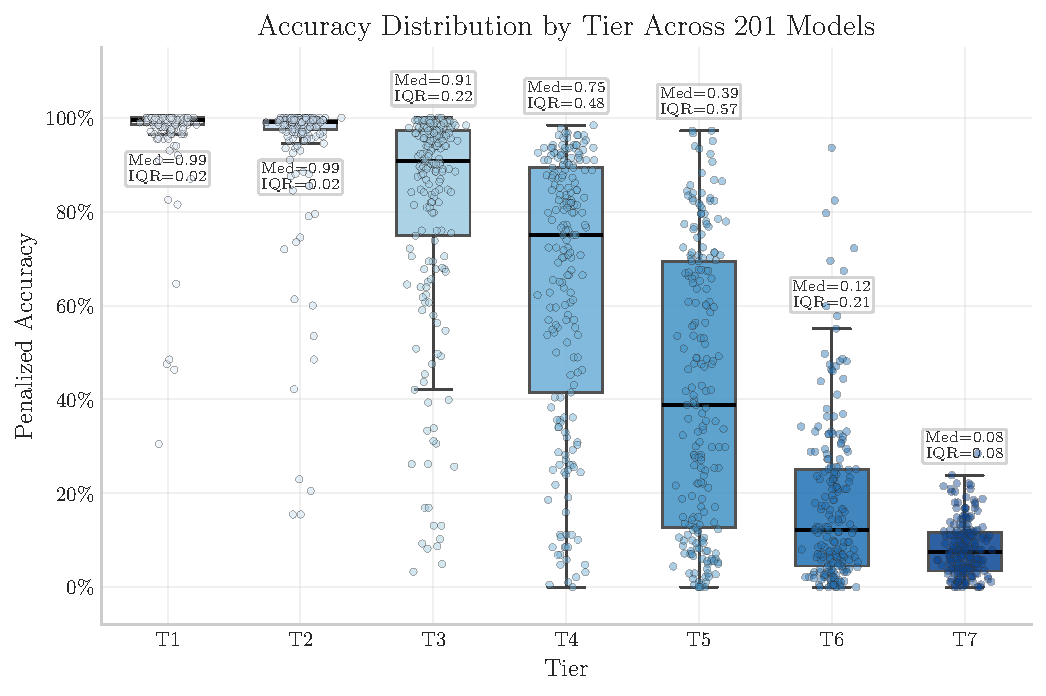
\includegraphics[width=0.85\textwidth]{figures/fig_a1_tier_boxplots.pdf}
    \caption{Accuracy distribution by tier across 188 models. T1--T2 are compressed at ceiling (median $>98\%$). T4 has the widest interquartile range, making it the best population discriminator. T6--T7 are at the floor for most models.}
    \label{fig:tier-boxplots}
\end{figure}

\begin{figure}[H]
    \centering
    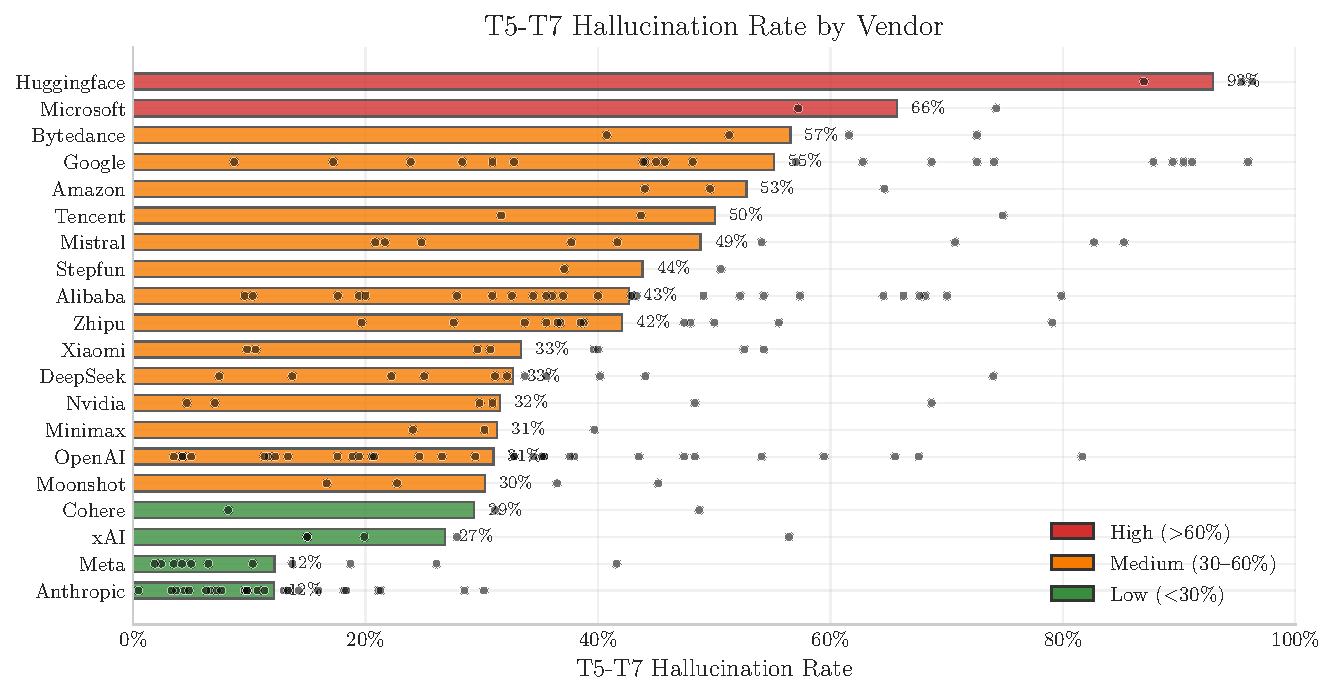
\includegraphics[width=\textwidth]{figures/fig_a2_vendor_hallucination.pdf}
    \caption{T5--T7 hallucination rate by vendor. Individual model points are overlaid on vendor means. Anthropic models hallucinate at only 10\% on probes beyond their knowledge (preferring to refuse), while Microsoft and Google models hallucinate at 58--66\%. This vendor-specific calibration directly impacts IKP scoring.}
    \label{fig:vendor-hallucination}
\end{figure}

\begin{landscape}
\small
\setlength{\tabcolsep}{4pt}
\begin{longtable}{@{}ll r r l c rr rrrrrrr@{}}
\caption{Full model results: per-tier accuracy. Models are grouped by vendor and sorted by penalized accuracy. The \textbf{IKP Pred.} column shows the calibration's predicted parameter count and ratio to actual for open-weight models; ratios $>2\times$ or $<0.5\times$ are bolded as systematic outliers. Above-trend outliers typically indicate denser training-data coverage or extra post-training; below-trend outliers typically indicate aggressive refusal policies (e.g., the small Llama instruction-tuned variants and Llama 4 Scout) or suboptimal training-data utilization. Proprietary models have no ground truth and show `--'.}
\label{tab:full-accuracy} \\
\toprule
\textbf{Vendor} & \textbf{Model} & \textbf{Params} & \textbf{IKP Pred.} & \textbf{Arch} & \textbf{Think} & \textbf{Acc.} & \textbf{Raw} & \textbf{T1} & \textbf{T2} & \textbf{T3} & \textbf{T4} & \textbf{T5} & \textbf{T6} & \textbf{T7} \\
\midrule
\endfirsthead
\toprule
\textbf{Vendor} & \textbf{Model} & \textbf{Params} & \textbf{IKP Pred.} & \textbf{Arch} & \textbf{Think} & \textbf{Acc.} & \textbf{Raw} & \textbf{T1} & \textbf{T2} & \textbf{T3} & \textbf{T4} & \textbf{T5} & \textbf{T6} & \textbf{T7} \\
\midrule
\endhead
\bottomrule
\endfoot
Google & gemini-3.1-pro & -- & -- & -- &  & 0.811 & 0.822 & 1.00 & 0.99 & 0.97 & 0.94 & 0.89 & 0.89 & 0.00 \\
 & gemini-3-flash-think & -- & -- & -- & Y & 0.756 & 0.809 & 1.00 & 0.99 & 0.97 & 0.87 & 0.88 & 0.58 & 0.00 \\
 & gemini-3-flash & -- & -- & -- &  & 0.745 & 0.804 & 1.00 & 1.00 & 0.95 & 0.87 & 0.85 & 0.54 & 0.00 \\
 & gemini-3.1-flash-lite & -- & -- & -- &  & 0.610 & 0.706 & 0.99 & 0.98 & 0.94 & 0.80 & 0.56 & 0.00 & 0.00 \\
 & gemini-2.5-pro & -- & -- & -- &  & 0.584 & 0.713 & 0.99 & 1.00 & 0.93 & 0.79 & 0.33 & 0.05 & 0.00 \\
 & gemini-2.5-pro-think & -- & -- & -- & Y & 0.579 & 0.710 & 0.98 & 1.00 & 0.92 & 0.74 & 0.41 & 0.00 & 0.00 \\
 & gemini-2.5-flash-think & -- & -- & -- & Y & 0.495 & 0.633 & 1.00 & 0.99 & 0.82 & 0.56 & 0.10 & 0.00 & 0.00 \\
 & gemini-2.0-flash & -- & -- & -- &  & 0.481 & 0.602 & 0.99 & 0.97 & 0.80 & 0.55 & 0.07 & 0.00 & 0.00 \\
 & gemini-2.5-flash & -- & -- & -- &  & 0.474 & 0.569 & 0.98 & 0.98 & 0.72 & 0.52 & 0.11 & 0.00 & 0.00 \\
 & gemini-2.5-flash-lite-think & -- & -- & -- & Y & 0.415 & 0.530 & 1.00 & 0.98 & 0.68 & 0.25 & 0.00 & 0.00 & 0.00 \\
 & gemini-2.5-flash-lite & -- & -- & -- &  & 0.401 & 0.506 & 0.98 & 0.97 & 0.66 & 0.20 & 0.00 & 0.00 & 0.00 \\
 & gemma-4-31b & 31B & 17B (0.5$\times$) & Dense &  & 0.313 & 0.423 & 0.99 & 0.98 & 0.21 & 0.00 & 0.00 & 0.00 & 0.00 \\
 & gemma-4-26b-a4b & 26B & 17B (0.6$\times$) & MoE &  & 0.312 & 0.420 & 0.99 & 0.96 & 0.23 & 0.00 & 0.00 & 0.00 & 0.00 \\
 & gemma-3-27b & 27B & 16B (0.6$\times$) & Dense &  & 0.309 & 0.421 & 0.98 & 0.96 & 0.23 & 0.00 & 0.00 & 0.00 & 0.00 \\
 & gemma-2-27b & 27B & 14B (0.5$\times$) & Dense &  & 0.300 & 0.396 & 0.98 & 0.91 & 0.21 & 0.00 & 0.00 & 0.00 & 0.00 \\
 & gemma-3-12b & 12B & 8B (0.6$\times$) & Dense &  & 0.261 & 0.369 & 0.96 & 0.87 & 0.00 & 0.00 & 0.00 & 0.00 & 0.00 \\
 & gemma-3n-e4b & 4B & 6B (1.5$\times$) & Dense &  & 0.247 & 0.321 & 0.98 & 0.75 & 0.00 & 0.00 & 0.00 & 0.00 & 0.00 \\
 & gemma-3-4b & 4B & 4B (1.0$\times$) & Dense &  & 0.220 & 0.296 & 0.96 & 0.58 & 0.00 & 0.00 & 0.00 & 0.00 & 0.00 \\
 & gemma-2-2b & 3B & 2B (0.9$\times$) & Dense &  & 0.189 & 0.266 & 0.88 & 0.45 & 0.00 & 0.00 & 0.00 & 0.00 & 0.00 \\
 & gemma-3-1b & 1B & 0.5B (0.5$\times$) & Dense &  & 0.091 & 0.202 & 0.64 & 0.00 & 0.00 & 0.00 & 0.00 & 0.00 & 0.00 \\
 & gemma-3-270m & 0.268B & 0.1B (0.5$\times$) & Dense &  & 0.001 & 0.072 & 0.01 & 0.00 & 0.00 & 0.00 & 0.00 & 0.00 & 0.00 \\
\midrule
OpenAI & gpt-5.5-pro & -- & -- & -- & Y & 0.723 & 0.796 & 1.00 & 1.00 & 0.94 & 0.92 & 0.76 & 0.45 & 0.00 \\
 & gpt-5.5-think & -- & -- & -- & Y & 0.719 & 0.782 & 1.00 & 1.00 & 0.94 & 0.89 & 0.78 & 0.43 & 0.00 \\
 & gpt-5.5 & -- & -- & -- &  & 0.714 & 0.780 & 1.00 & 1.00 & 0.95 & 0.88 & 0.78 & 0.39 & 0.00 \\
 & gpt-5-pro & -- & -- & -- &  & 0.665 & 0.733 & 1.00 & 0.98 & 0.97 & 0.86 & 0.69 & 0.15 & 0.00 \\
 & gpt-5-think & -- & -- & -- & Y & 0.664 & 0.727 & 0.99 & 0.99 & 0.95 & 0.84 & 0.71 & 0.15 & 0.00 \\
 & gpt-5 & -- & -- & -- &  & 0.661 & 0.724 & 0.99 & 0.99 & 0.96 & 0.82 & 0.67 & 0.19 & 0.00 \\
 & o1 & -- & -- & -- & Y & 0.654 & 0.700 & 0.98 & 1.00 & 0.92 & 0.89 & 0.62 & 0.17 & 0.00 \\
 & o3 & -- & -- & -- &  & 0.644 & 0.726 & 1.00 & 0.99 & 0.94 & 0.81 & 0.66 & 0.11 & 0.00 \\
 & gpt-5.4-pro & -- & -- & -- &  & 0.625 & 0.736 & 1.00 & 0.99 & 0.93 & 0.87 & 0.56 & 0.02 & 0.00 \\
 & gpt-4.1 & -- & -- & -- &  & 0.623 & 0.724 & 1.00 & 0.97 & 0.95 & 0.80 & 0.60 & 0.05 & 0.00 \\
 & gpt-5.3 & -- & -- & -- &  & 0.600 & 0.669 & 1.00 & 0.99 & 0.94 & 0.82 & 0.46 & 0.00 & 0.00 \\
 & gpt-5.2-pro & -- & -- & -- &  & 0.597 & 0.661 & 0.99 & 0.99 & 0.94 & 0.80 & 0.41 & 0.04 & 0.00 \\
 & gpt-5.1 & -- & -- & -- &  & 0.593 & 0.649 & 0.99 & 0.97 & 0.88 & 0.69 & 0.52 & 0.10 & 0.00 \\
 & gpt-5.2 & -- & -- & -- &  & 0.589 & 0.639 & 0.99 & 0.98 & 0.96 & 0.79 & 0.39 & 0.01 & 0.00 \\
 & gpt-5.4 & -- & -- & -- &  & 0.577 & 0.666 & 1.00 & 0.97 & 0.86 & 0.82 & 0.38 & 0.00 & 0.00 \\
 & gpt-4o & -- & -- & -- &  & 0.553 & 0.603 & 0.98 & 0.97 & 0.81 & 0.63 & 0.41 & 0.07 & 0.00 \\
 & gpt-4 & 1.8T & 666B (0.4$\times$) & MoE &  & 0.548 & 0.614 & 0.99 & 0.98 & 0.85 & 0.64 & 0.38 & 0.00 & 0.00 \\
 & gpt-4-turbo & -- & -- & -- &  & 0.545 & 0.610 & 0.99 & 1.00 & 0.85 & 0.67 & 0.30 & 0.00 & 0.00 \\
 & o4-mini-think & -- & -- & -- & Y & 0.527 & 0.617 & 1.00 & 0.99 & 0.89 & 0.66 & 0.15 & 0.00 & 0.00 \\
 & gpt-5-mini & -- & -- & -- &  & 0.517 & 0.534 & 0.99 & 0.99 & 0.84 & 0.57 & 0.19 & 0.03 & 0.00 \\
 & gpt-5-mini-think & -- & -- & -- & Y & 0.515 & 0.540 & 0.99 & 0.99 & 0.85 & 0.56 & 0.20 & 0.02 & 0.00 \\
 & gpt-5.4-mini & -- & -- & -- &  & 0.492 & 0.570 & 1.00 & 0.98 & 0.73 & 0.54 & 0.19 & 0.00 & 0.00 \\
 & gpt-4.1-mini & -- & -- & -- &  & 0.475 & 0.616 & 0.99 & 0.98 & 0.77 & 0.55 & 0.04 & 0.00 & 0.00 \\
 & gpt-3.5-turbo & -- & -- & -- &  & 0.469 & 0.551 & 0.99 & 0.98 & 0.76 & 0.39 & 0.16 & 0.00 & 0.00 \\
 & o3-mini & -- & -- & -- &  & 0.437 & 0.497 & 0.98 & 0.99 & 0.78 & 0.31 & 0.00 & 0.00 & 0.00 \\
 & gpt-5-nano-think & -- & -- & -- & Y & 0.417 & 0.441 & 1.00 & 0.99 & 0.63 & 0.30 & 0.00 & 0.00 & 0.00 \\
 & gpt-5-nano & -- & -- & -- &  & 0.405 & 0.431 & 0.99 & 0.96 & 0.63 & 0.25 & 0.00 & 0.00 & 0.00 \\
 & gpt-4o-mini & -- & -- & -- &  & 0.401 & 0.506 & 0.98 & 0.96 & 0.66 & 0.20 & 0.00 & 0.00 & 0.00 \\
 & gpt-oss-120b-think & 120B & 47B (0.4$\times$) & Dense & Y & 0.379 & 0.508 & 0.95 & 0.97 & 0.56 & 0.17 & 0.00 & 0.00 & 0.00 \\
 & gpt-4.1-nano & -- & -- & -- &  & 0.351 & 0.478 & 1.00 & 0.93 & 0.51 & 0.02 & 0.00 & 0.00 & 0.00 \\
 & gpt-5.4-nano & -- & -- & -- &  & 0.323 & 0.386 & 0.94 & 0.90 & 0.42 & 0.00 & 0.00 & 0.00 & 0.00 \\
 & gpt-oss-20b-think & 20B & 15B (0.7$\times$) & Dense & Y & 0.304 & 0.394 & 0.99 & 0.91 & 0.23 & 0.00 & 0.00 & 0.00 & 0.00 \\
\midrule
Anthropic & claude-opus-4.6-think & -- & -- & -- & Y & 0.680 & 0.741 & 1.00 & 1.00 & 0.97 & 0.93 & 0.70 & 0.17 & 0.00 \\
 & claude-opus-4.7-think & -- & -- & -- & Y & 0.664 & 0.714 & 1.00 & 0.98 & 0.96 & 0.90 & 0.68 & 0.13 & 0.00 \\
 & claude-opus-4.7 & -- & -- & -- &  & 0.657 & 0.688 & 1.00 & 0.98 & 0.93 & 0.89 & 0.66 & 0.14 & 0.00 \\
 & claude-opus-4.5-think & -- & -- & -- & Y & 0.652 & 0.682 & 1.00 & 1.00 & 0.98 & 0.86 & 0.61 & 0.11 & 0.00 \\
 & claude-opus-4.1-think & -- & -- & -- & Y & 0.649 & 0.681 & 0.98 & 1.00 & 0.98 & 0.86 & 0.58 & 0.13 & 0.00 \\
 & claude-opus-4.6 & -- & -- & -- &  & 0.631 & 0.689 & 1.00 & 0.99 & 0.96 & 0.89 & 0.57 & 0.00 & 0.00 \\
 & claude-sonnet-4.5-think & -- & -- & -- & Y & 0.614 & 0.654 & 0.99 & 1.00 & 0.95 & 0.84 & 0.51 & 0.00 & 0.00 \\
 & claude-opus-4.5 & -- & -- & -- &  & 0.611 & 0.654 & 0.99 & 0.98 & 0.94 & 0.79 & 0.51 & 0.06 & 0.00 \\
 & claude-sonnet-4.6-think & -- & -- & -- & Y & 0.609 & 0.682 & 0.99 & 0.99 & 0.92 & 0.84 & 0.52 & 0.00 & 0.00 \\
 & claude-opus-4-think & -- & -- & -- & Y & 0.597 & 0.621 & 0.99 & 0.99 & 0.95 & 0.72 & 0.43 & 0.07 & 0.00 \\
 & claude-sonnet-4.6 & -- & -- & -- &  & 0.582 & 0.638 & 1.00 & 1.00 & 0.92 & 0.82 & 0.33 & 0.00 & 0.00 \\
 & claude-opus-4.1 & -- & -- & -- &  & 0.579 & 0.599 & 0.99 & 1.00 & 0.91 & 0.69 & 0.40 & 0.06 & 0.00 \\
 & claude-sonnet-4.5 & -- & -- & -- &  & 0.550 & 0.577 & 0.99 & 1.00 & 0.90 & 0.65 & 0.31 & 0.00 & 0.00 \\
 & claude-3.7-sonnet & -- & -- & -- &  & 0.549 & 0.610 & 0.98 & 1.00 & 0.83 & 0.60 & 0.33 & 0.09 & 0.00 \\
 & claude-3.7-sonnet-think & -- & -- & -- & Y & 0.544 & 0.561 & 0.98 & 0.98 & 0.86 & 0.61 & 0.34 & 0.04 & 0.00 \\
 & claude-opus-4 & -- & -- & -- &  & 0.524 & 0.539 & 0.98 & 0.99 & 0.87 & 0.59 & 0.22 & 0.01 & 0.00 \\
 & claude-sonnet-4-think & -- & -- & -- & Y & 0.523 & 0.543 & 0.99 & 1.00 & 0.81 & 0.59 & 0.25 & 0.01 & 0.00 \\
 & claude-sonnet-4 & -- & -- & -- &  & 0.482 & 0.491 & 0.99 & 0.99 & 0.81 & 0.47 & 0.11 & 0.00 & 0.00 \\
 & claude-3.5-haiku & -- & -- & -- &  & 0.456 & 0.516 & 0.98 & 0.99 & 0.68 & 0.44 & 0.10 & 0.00 & 0.00 \\
 & claude-haiku-4.5-think & -- & -- & -- & Y & 0.432 & 0.483 & 0.97 & 0.99 & 0.73 & 0.34 & 0.00 & 0.00 & 0.00 \\
 & claude-haiku-4.5 & -- & -- & -- &  & 0.399 & 0.446 & 0.99 & 0.97 & 0.57 & 0.26 & 0.00 & 0.00 & 0.00 \\
 & claude-3-haiku & -- & -- & -- &  & 0.371 & 0.399 & 0.99 & 0.92 & 0.50 & 0.17 & 0.01 & 0.01 & 0.00 \\
\midrule
xAI & grok-4 & -- & -- & -- &  & 0.648 & 0.702 & 1.00 & 0.98 & 0.92 & 0.84 & 0.67 & 0.11 & 0.01 \\
 & grok-3 & -- & -- & -- &  & 0.623 & 0.691 & 1.00 & 1.00 & 0.93 & 0.83 & 0.57 & 0.03 & 0.00 \\
 & grok-4.20-think & -- & -- & -- & Y & 0.535 & 0.583 & 1.00 & 0.98 & 0.91 & 0.63 & 0.22 & 0.00 & 0.00 \\
 & grok-3-mini-think & -- & -- & -- & Y & 0.500 & 0.559 & 1.00 & 0.94 & 0.86 & 0.60 & 0.10 & 0.00 & 0.00 \\
 & grok-4.20 & -- & -- & -- &  & 0.432 & 0.519 & 1.00 & 0.95 & 0.72 & 0.35 & 0.00 & 0.00 & 0.00 \\
\midrule
Moonshot & kimi-k2.5-think & 1.0T & 3.0T (2.9$\times$) & MoE & Y & 0.644 & 0.684 & 0.99 & 0.99 & 0.94 & 0.92 & 0.67 & 0.00 & 0.00 \\
 & kimi-k2.6-think & 1.0T & 2.2T (2.1$\times$) & MoE & Y & 0.624 & 0.649 & 0.99 & 1.00 & 0.97 & 0.85 & 0.56 & 0.00 & 0.00 \\
 & kimi-k2 & 1.0T & 417B (0.4$\times$) & MoE &  & 0.518 & 0.584 & 0.99 & 0.99 & 0.84 & 0.57 & 0.24 & 0.00 & 0.00 \\
\midrule
Xiaomi & mimo-v2.5-pro-think & -- & -- & -- & Y & 0.615 & 0.691 & 1.00 & 0.99 & 0.95 & 0.82 & 0.55 & 0.00 & 0.00 \\
 & mimo-v2.5-pro & -- & -- & -- &  & 0.613 & 0.697 & 1.00 & 0.99 & 0.95 & 0.83 & 0.51 & 0.00 & 0.00 \\
 & mimo-v2-pro & -- & -- & -- &  & 0.586 & 0.619 & 0.99 & 1.00 & 0.93 & 0.72 & 0.39 & 0.08 & 0.00 \\
 & mimo-v2-pro-think & -- & -- & -- & Y & 0.576 & 0.616 & 0.98 & 0.99 & 0.92 & 0.72 & 0.40 & 0.03 & 0.00 \\
 & mimo-v2.5 & -- & -- & -- &  & 0.516 & 0.624 & 1.00 & 0.97 & 0.89 & 0.71 & 0.04 & 0.00 & 0.00 \\
 & mimo-v2.5-think & -- & -- & -- & Y & 0.514 & 0.614 & 1.00 & 0.99 & 0.94 & 0.65 & 0.02 & 0.00 & 0.00 \\
 & mimo-v2-flash & 309B & 151B (0.5$\times$) & MoE &  & 0.453 & 0.555 & 0.98 & 0.93 & 0.73 & 0.53 & 0.00 & 0.00 & 0.00 \\
 & mimo-v2-flash-think & 309B & 147B (0.5$\times$) & MoE & Y & 0.452 & 0.551 & 1.00 & 0.98 & 0.73 & 0.45 & 0.00 & 0.00 & 0.00 \\
\midrule
DeepSeek & deepseek-v4-pro-think & 1.6T & 1.8T (1.1$\times$) & MoE & Y & 0.613 & 0.705 & 1.00 & 0.99 & 0.90 & 0.86 & 0.53 & 0.01 & 0.00 \\
 & deepseek-v4-pro & 1.6T & 1.5T (0.9$\times$) & MoE &  & 0.599 & 0.647 & 0.98 & 0.97 & 0.92 & 0.79 & 0.46 & 0.07 & 0.00 \\
 & deepseek-v4-flash-think & 284B & 915B (3.2$\times$) & MoE & Y & 0.569 & 0.670 & 1.00 & 0.99 & 0.91 & 0.76 & 0.32 & 0.00 & 0.00 \\
 & deepseek-v4-flash & 284B & 832B (2.9$\times$) & MoE &  & 0.562 & 0.671 & 0.98 & 1.00 & 0.91 & 0.74 & 0.30 & 0.00 & 0.00 \\
 & deepseek-v3 & 671B & 589B (0.9$\times$) & MoE &  & 0.540 & 0.605 & 0.99 & 0.99 & 0.86 & 0.69 & 0.25 & 0.00 & 0.00 \\
 & deepseek-v3.2-think & 671B & 512B (0.8$\times$) & MoE & Y & 0.531 & 0.621 & 1.00 & 0.99 & 0.83 & 0.65 & 0.26 & 0.00 & 0.00 \\
 & deepseek-r1-think & 671B & 424B (0.6$\times$) & MoE & Y & 0.519 & 0.609 & 1.00 & 0.95 & 0.84 & 0.69 & 0.15 & 0.00 & 0.00 \\
 & deepseek-v3.2 & 671B & 335B (0.5$\times$) & MoE &  & 0.504 & 0.558 & 0.98 & 1.00 & 0.77 & 0.56 & 0.22 & 0.00 & 0.00 \\
 & deepseek-v3.1 & -- & -- & -- &  & 0.493 & 0.536 & 0.99 & 0.98 & 0.73 & 0.54 & 0.21 & 0.00 & 0.00 \\
 & deepseek-r1-distill-llama-70b-think & 70B & 57B (0.8$\times$) & Dense & Y & 0.391 & 0.509 & 0.97 & 0.93 & 0.62 & 0.21 & 0.00 & 0.00 & 0.00 \\
 & deepseek-r1-distill-qwen-32b-think & 32B & 14B (0.4$\times$) & Dense & Y & 0.302 & 0.383 & 0.96 & 0.91 & 0.24 & 0.00 & 0.00 & 0.00 & 0.00 \\
\midrule
Tencent & hy3-preview & -- & -- & -- &  & 0.581 & 0.666 & 1.00 & 0.99 & 0.93 & 0.76 & 0.39 & 0.00 & 0.00 \\
 & hunyuan-a13b & 80B & 5B (0.1$\times$) & MoE &  & 0.234 & 0.317 & 0.91 & 0.72 & 0.00 & 0.00 & 0.00 & 0.00 & 0.00 \\
 & hunyuan-a13b-think & 80B & 5B (0.1$\times$) & MoE & Y & 0.233 & 0.326 & 0.92 & 0.71 & 0.00 & 0.00 & 0.00 & 0.00 & 0.00 \\
\midrule
Zhipu & glm-5.1-think & 754B & 1.1T (1.4$\times$) & MoE & Y & 0.578 & 0.670 & 0.94 & 0.96 & 0.93 & 0.81 & 0.41 & 0.00 & 0.00 \\
 & glm-5-think & 744B & 910B (1.2$\times$) & MoE & Y & 0.568 & 0.658 & 0.97 & 0.98 & 0.91 & 0.76 & 0.34 & 0.00 & 0.00 \\
 & glm-5-turbo-think & -- & -- & -- & Y & 0.557 & 0.636 & 0.99 & 0.99 & 0.93 & 0.72 & 0.27 & 0.00 & 0.00 \\
 & glm-4.7-think & 358B & 692B (1.9$\times$) & MoE & Y & 0.551 & 0.657 & 0.99 & 0.98 & 0.89 & 0.76 & 0.24 & 0.00 & 0.00 \\
 & glm-4.5-think & 355B & 509B (1.4$\times$) & MoE & Y & 0.531 & 0.588 & 0.99 & 0.99 & 0.91 & 0.57 & 0.25 & 0.00 & 0.00 \\
 & glm-4.6-think & 357B & 366B (1.0$\times$) & MoE & Y & 0.510 & 0.636 & 0.99 & 0.97 & 0.82 & 0.69 & 0.10 & 0.00 & 0.00 \\
 & glm-4.5-air-think & 106B & 128B (1.2$\times$) & MoE & Y & 0.443 & 0.548 & 0.99 & 0.98 & 0.71 & 0.42 & 0.00 & 0.00 & 0.00 \\
 & glm-4.7-flash-think & 30B & 38B (1.3$\times$) & MoE & Y & 0.365 & 0.479 & 0.97 & 0.99 & 0.60 & 0.00 & 0.00 & 0.00 & 0.00 \\
 & glm-4-32b & 32B & 27B (0.8$\times$) & Dense &  & 0.342 & 0.461 & 0.96 & 0.96 & 0.44 & 0.04 & 0.00 & 0.00 & 0.00 \\
\midrule
Alibaba & qwen3.6-plus-think & -- & -- & -- & Y & 0.561 & 0.597 & 0.99 & 1.00 & 0.93 & 0.76 & 0.25 & 0.00 & 0.00 \\
 & qwen3-max & -- & -- & -- &  & 0.550 & 0.618 & 1.00 & 0.99 & 0.90 & 0.67 & 0.30 & 0.00 & 0.00 \\
 & qwen3.5-plus-think & -- & -- & -- & Y & 0.493 & 0.585 & 0.99 & 0.98 & 0.84 & 0.63 & 0.00 & 0.00 & 0.00 \\
 & qwen3.5-397b-a17b-think & 397B & 264B (0.7$\times$) & MoE & Y & 0.489 & 0.584 & 0.99 & 0.98 & 0.79 & 0.58 & 0.09 & 0.00 & 0.00 \\
 & qwen3.5-122b-a10b-think & 122B & 241B (2.0$\times$) & MoE & Y & 0.483 & 0.559 & 0.99 & 0.98 & 0.85 & 0.56 & 0.00 & 0.00 & 0.00 \\
 & qwen-plus & -- & -- & -- &  & 0.474 & 0.555 & 0.97 & 0.99 & 0.81 & 0.51 & 0.03 & 0.00 & 0.00 \\
 & qwen3-next-80b-a3b & 80B & 127B (1.6$\times$) & MoE &  & 0.442 & 0.520 & 0.97 & 0.99 & 0.78 & 0.36 & 0.00 & 0.00 & 0.00 \\
 & qwen3-235b-a22b-think & 235B & 114B (0.5$\times$) & MoE & Y & 0.435 & 0.513 & 0.98 & 0.98 & 0.70 & 0.38 & 0.00 & 0.00 & 0.00 \\
 & qwen-max & -- & -- & -- &  & 0.418 & 0.482 & 0.98 & 0.98 & 0.66 & 0.30 & 0.00 & 0.00 & 0.00 \\
 & qwen3.5-flash-think & -- & -- & -- & Y & 0.383 & 0.486 & 1.00 & 0.98 & 0.64 & 0.06 & 0.00 & 0.00 & 0.00 \\
 & qwen-2.5-72b & 73B & 50B (0.7$\times$) & Dense &  & 0.382 & 0.466 & 1.00 & 0.98 & 0.59 & 0.10 & 0.00 & 0.00 & 0.00 \\
 & qwen3.5-35b-a3b-think & 35B & 43B (1.2$\times$) & MoE & Y & 0.374 & 0.477 & 0.99 & 0.95 & 0.67 & 0.00 & 0.00 & 0.00 & 0.00 \\
 & qwen3.5-27b-think & 27B & 35B (1.3$\times$) & Dense & Y & 0.360 & 0.466 & 0.99 & 0.95 & 0.58 & 0.00 & 0.00 & 0.00 & 0.00 \\
 & qwen3-32b-think & 32B & 34B (1.1$\times$) & Dense & Y & 0.359 & 0.421 & 0.98 & 0.94 & 0.59 & 0.00 & 0.00 & 0.00 & 0.00 \\
 & qwen3-30b-a3b-think & 30B & 27B (0.9$\times$) & MoE & Y & 0.342 & 0.414 & 0.98 & 0.96 & 0.45 & 0.00 & 0.00 & 0.00 & 0.00 \\
 & qwq-32b-think & 32B & 26B (0.8$\times$) & Dense &  & 0.340 & 0.435 & 0.99 & 0.94 & 0.45 & 0.00 & 0.00 & 0.00 & 0.00 \\
 & qwen3-14b-think & 14B & 19B (1.3$\times$) & Dense & Y & 0.320 & 0.399 & 0.95 & 0.94 & 0.35 & 0.00 & 0.00 & 0.00 & 0.00 \\
 & qwen3.5-9b-think & 9B & 14B (1.6$\times$) & Dense & Y & 0.301 & 0.392 & 0.98 & 0.92 & 0.20 & 0.00 & 0.00 & 0.00 & 0.00 \\
 & qwen-turbo & -- & -- & -- &  & 0.294 & 0.384 & 0.92 & 0.93 & 0.21 & 0.00 & 0.00 & 0.00 & 0.00 \\
 & qwen-2.5-7b & 8B & 9B (1.2$\times$) & Dense &  & 0.273 & 0.321 & 0.96 & 0.94 & 0.00 & 0.00 & 0.00 & 0.00 & 0.00 \\
 & qwen3-8b-think & 8B & 8B (1.0$\times$) & Dense & Y & 0.264 & 0.363 & 0.96 & 0.89 & 0.00 & 0.00 & 0.00 & 0.00 & 0.00 \\
 & qwen-2.5-0.5b & 0.494B & 0.9B (1.8$\times$) & Dense &  & 0.126 & 0.165 & 0.88 & 0.00 & 0.00 & 0.00 & 0.00 & 0.00 & 0.00 \\
 & qwen3.5-0.8b & 0.8B & 0.3B (0.3$\times$) & Dense &  & 0.046 & 0.073 & 0.25 & 0.07 & 0.00 & 0.00 & 0.00 & 0.00 & 0.00 \\
 & qwen3-0.6b & 0.596B & 0.2B (0.3$\times$) & Dense &  & 0.026 & 0.105 & 0.18 & 0.00 & 0.00 & 0.00 & 0.00 & 0.00 & 0.00 \\
\midrule
NVIDIA & nemotron-70b & 70B & 490B (7.0$\times$) & Dense &  & 0.529 & 0.575 & 0.99 & 0.99 & 0.83 & 0.67 & 0.21 & 0.00 & 0.00 \\
 & nemotron-3-super-120b & 120B & 135B (1.1$\times$) & MoE &  & 0.446 & 0.550 & 0.99 & 0.97 & 0.77 & 0.39 & 0.00 & 0.00 & 0.00 \\
 & nemotron-super-49b-think & 49B & 19B (0.4$\times$) & Dense & Y & 0.320 & 0.414 & 0.96 & 0.98 & 0.29 & 0.00 & 0.00 & 0.00 & 0.00 \\
 & nemotron-3-nano-30b & 30B & 16B (0.5$\times$) & MoE &  & 0.309 & 0.407 & 0.99 & 0.96 & 0.21 & 0.00 & 0.00 & 0.00 & 0.00 \\
 & nemotron-nano-9b-v2 & 9B & 13B (1.4$\times$) & Dense &  & 0.295 & 0.334 & 0.97 & 0.84 & 0.26 & 0.00 & 0.00 & 0.00 & 0.00 \\
\midrule
ByteDance & seed-2.0-lite-think & -- & -- & -- & Y & 0.526 & 0.621 & 1.00 & 0.99 & 0.87 & 0.74 & 0.08 & 0.00 & 0.00 \\
 & seed-1.6-think & -- & -- & -- & Y & 0.451 & 0.549 & 0.99 & 0.99 & 0.78 & 0.39 & 0.00 & 0.00 & 0.00 \\
 & seed-2.0-mini-think & -- & -- & -- & Y & 0.423 & 0.546 & 0.99 & 0.95 & 0.66 & 0.36 & 0.00 & 0.00 & 0.00 \\
 & seed-1.6-flash-think & -- & -- & -- & Y & 0.325 & 0.421 & 1.00 & 0.93 & 0.34 & 0.00 & 0.00 & 0.00 & 0.00 \\
\midrule
Meta & llama-4-maverick & 402B & 468B (1.2$\times$) & MoE &  & 0.526 & 0.613 & 0.98 & 0.99 & 0.79 & 0.64 & 0.26 & 0.02 & 0.00 \\
 & llama-3.1-70b & 71B & 293B (4.2$\times$) & Dense &  & 0.496 & 0.531 & 0.98 & 0.98 & 0.78 & 0.54 & 0.18 & 0.00 & 0.00 \\
 & hermes-4-405b & 405B & 288B (0.7$\times$) & Dense &  & 0.495 & 0.518 & 0.99 & 0.96 & 0.77 & 0.57 & 0.14 & 0.03 & 0.00 \\
 & llama-3.3-70b & 71B & 251B (3.5$\times$) & Dense &  & 0.486 & 0.567 & 0.96 & 0.99 & 0.70 & 0.57 & 0.18 & 0.00 & 0.00 \\
 & llama-3-70b & 71B & 139B (2.0$\times$) & Dense &  & 0.448 & 0.501 & 0.98 & 0.97 & 0.66 & 0.40 & 0.12 & 0.00 & 0.00 \\
 & hermes-3-405b & 405B & 119B (0.3$\times$) & Dense &  & 0.438 & 0.458 & 0.99 & 0.96 & 0.67 & 0.37 & 0.06 & 0.01 & 0.00 \\
 & llama-3.1-8b & 8B & 25B (3.1$\times$) & Dense &  & 0.338 & 0.394 & 0.96 & 0.93 & 0.37 & 0.10 & 0.00 & 0.00 & 0.00 \\
 & llama-4-scout & 109B & 18B (0.2$\times$) & MoE &  & 0.318 & 0.452 & 0.96 & 0.86 & 0.40 & 0.00 & 0.00 & 0.00 & 0.00 \\
 & llama-3-8b & 8B & 14B (1.8$\times$) & Dense &  & 0.301 & 0.412 & 0.96 & 0.92 & 0.23 & 0.00 & 0.00 & 0.00 & 0.00 \\
 & llama-3.2-3b & 3B & 7B (2.3$\times$) & Dense &  & 0.260 & 0.316 & 0.94 & 0.81 & 0.08 & 0.00 & 0.00 & 0.00 & 0.00 \\
 & llama-3.2-1b & 1B & 2B (1.5$\times$) & Dense &  & 0.171 & 0.236 & 0.79 & 0.41 & 0.00 & 0.00 & 0.00 & 0.00 & 0.00 \\
\midrule
Mistral & mistral-medium-3.1 & -- & -- & -- &  & 0.520 & 0.566 & 0.98 & 0.97 & 0.82 & 0.68 & 0.19 & 0.00 & 0.00 \\
 & mistral-large & 123B & 198B (1.6$\times$) & Dense &  & 0.471 & 0.515 & 0.96 & 0.96 & 0.76 & 0.48 & 0.13 & 0.00 & 0.00 \\
 & mixtral-8x22b & 141B & 176B (1.3$\times$) & MoE &  & 0.463 & 0.529 & 0.99 & 1.00 & 0.71 & 0.48 & 0.07 & 0.00 & 0.00 \\
 & mistral-small-24b & 24B & 62B (2.6$\times$) & Dense &  & 0.397 & 0.452 & 0.98 & 0.98 & 0.61 & 0.20 & 0.00 & 0.00 & 0.00 \\
 & mixtral-8x7b & 47B & 40B (0.9$\times$) & MoE &  & 0.369 & 0.498 & 0.94 & 0.96 & 0.55 & 0.13 & 0.00 & 0.00 & 0.00 \\
 & ministral-8b & 8B & 13B (1.6$\times$) & Dense &  & 0.296 & 0.405 & 0.94 & 0.94 & 0.19 & 0.00 & 0.00 & 0.00 & 0.00 \\
 & mistral-nemo-12b & 12B & 10B (0.9$\times$) & Dense &  & 0.281 & 0.405 & 0.94 & 0.90 & 0.14 & 0.00 & 0.00 & 0.00 & 0.00 \\
 & ministral-3b & 3B & 6B (1.9$\times$) & Dense &  & 0.243 & 0.329 & 0.93 & 0.77 & 0.00 & 0.00 & 0.00 & 0.00 & 0.00 \\
 & mistral-7b & 7B & 5B (0.7$\times$) & Dense &  & 0.235 & 0.349 & 0.87 & 0.78 & 0.00 & 0.00 & 0.00 & 0.00 & 0.00 \\
\midrule
Ai21 & jamba-large & 398B & 370B (0.9$\times$) & MoE &  & 0.511 & 0.549 & 0.99 & 0.98 & 0.86 & 0.54 & 0.17 & 0.01 & 0.03 \\
\midrule
Amazon & nova-premier & -- & -- & -- &  & 0.487 & 0.593 & 1.00 & 0.97 & 0.83 & 0.61 & 0.00 & 0.00 & 0.00 \\
 & nova-pro & -- & -- & -- &  & 0.407 & 0.512 & 0.98 & 0.98 & 0.66 & 0.22 & 0.00 & 0.00 & 0.00 \\
 & nova-micro & -- & -- & -- &  & 0.274 & 0.377 & 0.98 & 0.89 & 0.05 & 0.00 & 0.00 & 0.00 & 0.00 \\
\midrule
Cohere & command-a & 111B & 223B (2.0$\times$) & Dense &  & 0.478 & 0.557 & 0.99 & 0.99 & 0.78 & 0.52 & 0.07 & 0.00 & 0.00 \\
 & command-r-plus & 104B & 52B (0.5$\times$) & Dense &  & 0.385 & 0.441 & 0.98 & 0.93 & 0.51 & 0.23 & 0.04 & 0.00 & 0.00 \\
 & command-r7b & 7B & 5B (0.7$\times$) & Dense &  & 0.232 & 0.336 & 0.93 & 0.69 & 0.00 & 0.00 & 0.00 & 0.00 & 0.00 \\
\midrule
Stepfun & step-3.5-flash-think & 197B & 183B (0.9$\times$) & MoE & Y & 0.466 & 0.595 & 1.00 & 0.97 & 0.79 & 0.50 & 0.00 & 0.00 & 0.00 \\
\midrule
Baidu & ernie-4.5-300b-a47b & 300B & 137B (0.5$\times$) & MoE &  & 0.447 & 0.499 & 0.98 & 0.97 & 0.70 & 0.36 & 0.12 & 0.00 & 0.00 \\
\midrule
MiniMax & minimax-m2.7-think & 230B & 75B (0.3$\times$) & MoE & Y & 0.409 & 0.475 & 0.97 & 0.98 & 0.66 & 0.24 & 0.00 & 0.00 & 0.00 \\
 & minimax-m1-think & 456B & 0.8B (0.0$\times$) & MoE & Y & 0.114 & 0.342 & 0.30 & 0.23 & 0.27 & 0.00 & 0.00 & 0.00 & 0.00 \\
\midrule
Nex-Agi & deepseek-v3.1-nex-n1 & 671B & 40B (0.1$\times$) & MoE &  & 0.369 & 0.381 & 0.98 & 0.95 & 0.46 & 0.17 & 0.01 & 0.00 & 0.00 \\
\midrule
Prime-Intellect & intellect-3-think & 106B & 22B (0.2$\times$) & MoE & Y & 0.329 & 0.479 & 0.97 & 0.93 & 0.40 & 0.00 & 0.00 & 0.00 & 0.00 \\
\midrule
Microsoft & phi-4 & 15B & 15B (1.0$\times$) & Dense &  & 0.304 & 0.394 & 0.95 & 0.93 & 0.24 & 0.00 & 0.00 & 0.00 & 0.00 \\
 & phi-3-mini & 4B & 2B (0.6$\times$) & Dense &  & 0.190 & 0.281 & 0.85 & 0.48 & 0.00 & 0.00 & 0.00 & 0.00 & 0.00 \\
\midrule
AllenAI & olmo-3.1-32b & 32B & 14B (0.4$\times$) & Dense &  & 0.301 & 0.373 & 0.97 & 0.95 & 0.18 & 0.00 & 0.00 & 0.00 & 0.00 \\
\midrule
HuggingFace & smollm2-1.7b & 2B & 4B (2.1$\times$) & Dense &  & 0.214 & 0.280 & 0.91 & 0.59 & 0.00 & 0.00 & 0.00 & 0.00 & 0.00 \\
 & smollm2-360m & 0.362B & 0.6B (1.8$\times$) & Dense &  & 0.104 & 0.209 & 0.65 & 0.07 & 0.00 & 0.00 & 0.00 & 0.00 & 0.00 \\
 & smollm2-135m & 0.135B & 0.1B (0.9$\times$) & Dense &  & 0.000 & 0.117 & 0.00 & 0.00 & 0.00 & 0.00 & 0.00 & 0.00 & 0.00 \\
\midrule
Ibm & granite-3.3-2b & 2B & 2B (1.2$\times$) & Dense &  & 0.188 & 0.276 & 0.82 & 0.49 & 0.00 & 0.00 & 0.00 & 0.00 & 0.00 \\
\midrule
Inclusionai & ling-2.6-flash & 104B & 1B (0.0$\times$) & MoE &  & 0.137 & 0.184 & 0.39 & 0.39 & 0.17 & 0.01 & 0.00 & 0.00 & 0.00 \\
\end{longtable}

\end{landscape}

\begin{landscape}
\begin{longtable}{@{}ll rr rrrrrrr@{}}
\caption{Per-tier hallucination rates. Hallucination rate = wrong answers / (wrong + correct + refusal). Higher values indicate more confident incorrect responses. Models sorted as in Table~\ref{tab:full-accuracy}.}
\label{tab:full-hallucination} \\
\toprule
\textbf{Vendor} & \textbf{Model} & \textbf{Acc.} & \textbf{Raw} & \textbf{T1} & \textbf{T2} & \textbf{T3} & \textbf{T4} & \textbf{T5} & \textbf{T6} & \textbf{T7} \\
\midrule
\endfirsthead
\toprule
\textbf{Vendor} & \textbf{Model} & \textbf{Acc.} & \textbf{Raw} & \textbf{T1} & \textbf{T2} & \textbf{T3} & \textbf{T4} & \textbf{T5} & \textbf{T6} & \textbf{T7} \\
\midrule
\endhead
\bottomrule
\endfoot
Google & gemini-3.1-pro & 0.811 & 0.822 & 0.00 & 0.01 & 0.01 & 0.02 & 0.03 & 0.03 & 0.23 \\
 & gemini-3-flash-think & 0.756 & 0.809 & 0.00 & 0.01 & 0.01 & 0.06 & 0.04 & 0.20 & 0.73 \\
 & gemini-3-flash & 0.745 & 0.804 & 0.00 & 0.00 & 0.02 & 0.05 & 0.06 & 0.21 & 0.58 \\
 & gemini-3.1-flash-lite & 0.610 & 0.706 & 0.00 & 0.01 & 0.03 & 0.09 & 0.17 & 0.46 & 0.67 \\
 & gemini-2.5-pro & 0.584 & 0.713 & 0.01 & 0.00 & 0.03 & 0.09 & 0.31 & 0.45 & 0.80 \\
 & gemini-2.5-pro-think & 0.579 & 0.710 & 0.01 & 0.00 & 0.03 & 0.12 & 0.27 & 0.49 & 0.73 \\
 & gemini-2.5-flash-think & 0.495 & 0.633 & 0.00 & 0.01 & 0.08 & 0.21 & 0.41 & 0.61 & 0.67 \\
 & gemini-2.0-flash & 0.481 & 0.602 & 0.01 & 0.01 & 0.10 & 0.20 & 0.34 & 0.60 & 0.58 \\
 & gemini-2.5-flash & 0.474 & 0.569 & 0.01 & 0.01 & 0.11 & 0.19 & 0.18 & 0.19 & 0.20 \\
 & gemini-2.5-flash-lite-think & 0.415 & 0.530 & 0.00 & 0.01 & 0.14 & 0.36 & 0.72 & 0.81 & 0.83 \\
 & gemini-2.5-flash-lite & 0.401 & 0.506 & 0.01 & 0.01 & 0.11 & 0.30 & 0.29 & 0.53 & 0.38 \\
 & gemma-4-31b & 0.313 & 0.423 & 0.00 & 0.01 & 0.38 & 0.57 & 0.62 & 0.54 & 0.58 \\
 & gemma-4-26b-a4b & 0.312 & 0.420 & 0.01 & 0.01 & 0.35 & 0.54 & 0.56 & 0.54 & 0.46 \\
 & gemma-3-27b & 0.309 & 0.421 & 0.01 & 0.02 & 0.37 & 0.70 & 0.83 & 0.91 & 0.88 \\
 & gemma-2-27b & 0.300 & 0.396 & 0.01 & 0.04 & 0.37 & 0.66 & 0.69 & 0.45 & 0.52 \\
 & gemma-3-12b & 0.261 & 0.369 & 0.01 & 0.07 & 0.48 & 0.69 & 0.69 & 0.78 & 0.70 \\
 & gemma-3n-e4b & 0.247 & 0.321 & 0.01 & 0.12 & 0.68 & 0.91 & 0.87 & 0.81 & 0.56 \\
 & gemma-3-4b & 0.220 & 0.296 & 0.02 & 0.21 & 0.73 & 0.85 & 0.73 & 0.83 & 0.68 \\
 & gemma-2-2b & 0.189 & 0.266 & 0.06 & 0.28 & 0.84 & 0.91 & 0.91 & 0.71 & 0.88 \\
 & gemma-3-1b & 0.091 & 0.202 & 0.17 & 0.51 & 0.89 & 0.97 & 0.97 & 0.97 & 0.96 \\
 & gemma-3-270m & 0.001 & 0.072 & 0.29 & 0.35 & 0.48 & 0.33 & 0.14 & 0.16 & 0.28 \\
\midrule
OpenAI & gpt-5.5-pro & 0.723 & 0.796 & 0.00 & 0.00 & 0.03 & 0.03 & 0.10 & 0.27 & 0.69 \\
 & gpt-5.5-think & 0.719 & 0.782 & 0.00 & 0.00 & 0.03 & 0.04 & 0.07 & 0.23 & 0.47 \\
 & gpt-5.5 & 0.714 & 0.780 & 0.00 & 0.00 & 0.02 & 0.04 & 0.08 & 0.28 & 0.59 \\
 & gpt-5-pro & 0.665 & 0.733 & 0.00 & 0.01 & 0.01 & 0.04 & 0.06 & 0.30 & 0.32 \\
 & gpt-5-think & 0.664 & 0.727 & 0.00 & 0.01 & 0.01 & 0.06 & 0.03 & 0.27 & 0.28 \\
 & gpt-5 & 0.661 & 0.724 & 0.00 & 0.01 & 0.01 & 0.07 & 0.04 & 0.24 & 0.26 \\
 & o1 & 0.654 & 0.700 & 0.01 & 0.00 & 0.03 & 0.04 & 0.06 & 0.14 & 0.18 \\
 & o3 & 0.644 & 0.726 & 0.00 & 0.01 & 0.02 & 0.08 & 0.07 & 0.32 & 0.34 \\
 & gpt-5.4-pro & 0.625 & 0.736 & 0.00 & 0.01 & 0.03 & 0.06 & 0.19 & 0.45 & 0.64 \\
 & gpt-4.1 & 0.623 & 0.724 & 0.00 & 0.01 & 0.02 & 0.09 & 0.13 & 0.39 & 0.51 \\
 & gpt-5.3 & 0.600 & 0.669 & 0.00 & 0.01 & 0.02 & 0.06 & 0.13 & 0.26 & 0.31 \\
 & gpt-5.2-pro & 0.597 & 0.661 & 0.00 & 0.01 & 0.03 & 0.07 & 0.12 & 0.20 & 0.23 \\
 & gpt-5.1 & 0.593 & 0.649 & 0.00 & 0.01 & 0.04 & 0.12 & 0.07 & 0.14 & 0.16 \\
 & gpt-5.2 & 0.589 & 0.639 & 0.00 & 0.01 & 0.01 & 0.07 & 0.12 & 0.18 & 0.21 \\
 & gpt-5.4 & 0.577 & 0.666 & 0.00 & 0.01 & 0.06 & 0.07 & 0.20 & 0.38 & 0.44 \\
 & gpt-4o & 0.553 & 0.603 & 0.01 & 0.01 & 0.04 & 0.06 & 0.03 & 0.15 & 0.17 \\
 & gpt-4 & 0.548 & 0.614 & 0.01 & 0.01 & 0.04 & 0.09 & 0.09 & 0.24 & 0.21 \\
 & gpt-4-turbo & 0.545 & 0.610 & 0.00 & 0.00 & 0.03 & 0.07 & 0.11 & 0.49 & 0.41 \\
 & o4-mini-think & 0.527 & 0.617 & 0.00 & 0.01 & 0.04 & 0.12 & 0.20 & 0.34 & 0.31 \\
 & gpt-5-mini & 0.517 & 0.534 & 0.00 & 0.00 & 0.02 & 0.04 & 0.01 & 0.03 & 0.06 \\
 & gpt-5-mini-think & 0.515 & 0.540 & 0.00 & 0.01 & 0.03 & 0.05 & 0.03 & 0.04 & 0.05 \\
 & gpt-5.4-mini & 0.492 & 0.570 & 0.00 & 0.01 & 0.09 & 0.15 & 0.16 & 0.45 & 0.28 \\
 & gpt-4.1-mini & 0.475 & 0.616 & 0.01 & 0.01 & 0.10 & 0.20 & 0.38 & 0.64 & 0.57 \\
 & gpt-3.5-turbo & 0.469 & 0.551 & 0.01 & 0.01 & 0.06 & 0.18 & 0.17 & 0.56 & 0.43 \\
 & o3-mini & 0.437 & 0.497 & 0.01 & 0.01 & 0.06 & 0.21 & 0.24 & 0.20 & 0.23 \\
 & gpt-5-nano-think & 0.417 & 0.441 & 0.00 & 0.01 & 0.05 & 0.08 & 0.03 & 0.03 & 0.07 \\
 & gpt-5-nano & 0.405 & 0.431 & 0.01 & 0.01 & 0.03 & 0.10 & 0.06 & 0.01 & 0.07 \\
 & gpt-4o-mini & 0.401 & 0.506 & 0.01 & 0.02 & 0.12 & 0.32 & 0.30 & 0.62 & 0.45 \\
 & gpt-oss-120b-think & 0.379 & 0.508 & 0.01 & 0.01 & 0.18 & 0.34 & 0.31 & 0.47 & 0.35 \\
 & gpt-4.1-nano & 0.351 & 0.478 & 0.00 & 0.04 & 0.22 & 0.43 & 0.38 & 0.68 & 0.47 \\
 & gpt-5.4-nano & 0.323 & 0.386 & 0.01 & 0.03 & 0.11 & 0.23 & 0.11 & 0.14 & 0.15 \\
 & gpt-oss-20b-think & 0.304 & 0.394 & 0.01 & 0.04 & 0.34 & 0.65 & 0.65 & 0.69 & 0.52 \\
\midrule
Anthropic & claude-opus-4.6-think & 0.680 & 0.741 & 0.00 & 0.00 & 0.01 & 0.03 & 0.10 & 0.25 & 0.28 \\
 & claude-opus-4.7-think & 0.664 & 0.714 & 0.00 & 0.01 & 0.01 & 0.04 & 0.07 & 0.17 & 0.15 \\
 & claude-opus-4.7 & 0.657 & 0.688 & 0.00 & 0.01 & 0.03 & 0.04 & 0.05 & 0.10 & 0.14 \\
 & claude-opus-4.5-think & 0.652 & 0.682 & 0.00 & 0.00 & 0.01 & 0.04 & 0.06 & 0.11 & 0.25 \\
 & claude-opus-4.1-think & 0.649 & 0.681 & 0.01 & 0.00 & 0.01 & 0.04 & 0.07 & 0.11 & 0.17 \\
 & claude-opus-4.6 & 0.631 & 0.689 & 0.00 & 0.00 & 0.01 & 0.04 & 0.07 & 0.28 & 0.27 \\
 & claude-sonnet-4.5-think & 0.614 & 0.654 & 0.00 & 0.00 & 0.02 & 0.05 & 0.09 & 0.17 & 0.16 \\
 & claude-opus-4.5 & 0.611 & 0.654 & 0.00 & 0.01 & 0.01 & 0.06 & 0.07 & 0.15 & 0.23 \\
 & claude-sonnet-4.6-think & 0.609 & 0.682 & 0.00 & 0.01 & 0.04 & 0.07 & 0.15 & 0.34 & 0.29 \\
 & claude-opus-4-think & 0.597 & 0.621 & 0.00 & 0.00 & 0.01 & 0.05 & 0.05 & 0.07 & 0.11 \\
 & claude-sonnet-4.6 & 0.582 & 0.638 & 0.00 & 0.00 & 0.03 & 0.06 & 0.14 & 0.40 & 0.28 \\
 & claude-opus-4.1 & 0.579 & 0.599 & 0.00 & 0.00 & 0.02 & 0.05 & 0.01 & 0.06 & 0.13 \\
 & claude-sonnet-4.5 & 0.550 & 0.577 & 0.00 & 0.00 & 0.02 & 0.06 & 0.04 & 0.07 & 0.12 \\
 & claude-3.7-sonnet & 0.549 & 0.610 & 0.01 & 0.00 & 0.04 & 0.10 & 0.07 & 0.17 & 0.18 \\
 & claude-3.7-sonnet-think & 0.544 & 0.561 & 0.01 & 0.01 & 0.01 & 0.06 & 0.01 & 0.04 & 0.08 \\
 & claude-opus-4 & 0.524 & 0.539 & 0.01 & 0.01 & 0.01 & 0.04 & 0.01 & 0.04 & 0.08 \\
 & claude-sonnet-4-think & 0.523 & 0.543 & 0.00 & 0.00 & 0.04 & 0.06 & 0.02 & 0.06 & 0.07 \\
 & claude-sonnet-4 & 0.482 & 0.491 & 0.00 & 0.01 & 0.00 & 0.05 & 0.01 & 0.04 & 0.07 \\
 & claude-3.5-haiku & 0.456 & 0.516 & 0.01 & 0.01 & 0.10 & 0.16 & 0.15 & 0.08 & 0.08 \\
 & claude-haiku-4.5-think & 0.432 & 0.483 & 0.01 & 0.01 & 0.07 & 0.15 & 0.13 & 0.07 & 0.09 \\
 & claude-haiku-4.5 & 0.399 & 0.446 & 0.01 & 0.01 & 0.09 & 0.13 & 0.10 & 0.12 & 0.09 \\
 & claude-3-haiku & 0.371 & 0.399 & 0.01 & 0.04 & 0.07 & 0.07 & 0.01 & 0.00 & 0.01 \\
\midrule
xAI & grok-4 & 0.648 & 0.702 & 0.00 & 0.01 & 0.03 & 0.06 & 0.09 & 0.21 & 0.07 \\
 & grok-3 & 0.623 & 0.691 & 0.00 & 0.00 & 0.03 & 0.07 & 0.12 & 0.30 & 0.12 \\
 & grok-4.20-think & 0.535 & 0.583 & 0.00 & 0.01 & 0.03 & 0.10 & 0.12 & 0.15 & 0.04 \\
 & grok-3-mini-think & 0.500 & 0.559 & 0.00 & 0.03 & 0.05 & 0.14 & 0.18 & 0.20 & 0.07 \\
 & grok-4.20 & 0.432 & 0.519 & 0.00 & 0.03 & 0.10 & 0.24 & 0.28 & 0.51 & 0.10 \\
\midrule
Moonshot & kimi-k2.5-think & 0.644 & 0.684 & 0.00 & 0.01 & 0.03 & 0.04 & 0.10 & 0.54 & 0.36 \\
 & kimi-k2.6-think & 0.624 & 0.649 & 0.01 & 0.00 & 0.01 & 0.03 & 0.03 & 0.26 & 0.17 \\
 & kimi-k2 & 0.518 & 0.584 & 0.01 & 0.01 & 0.06 & 0.16 & 0.14 & 0.24 & 0.07 \\
\midrule
Xiaomi & mimo-v2.5-pro-think & 0.615 & 0.691 & 0.00 & 0.01 & 0.02 & 0.07 & 0.17 & 0.45 & 0.46 \\
 & mimo-v2.5-pro & 0.613 & 0.697 & 0.00 & 0.01 & 0.02 & 0.07 & 0.20 & 0.41 & 0.47 \\
 & mimo-v2-pro & 0.586 & 0.619 & 0.01 & 0.00 & 0.01 & 0.07 & 0.11 & 0.07 & 0.15 \\
 & mimo-v2-pro-think & 0.576 & 0.616 & 0.01 & 0.01 & 0.02 & 0.08 & 0.09 & 0.10 & 0.17 \\
 & mimo-v2.5 & 0.516 & 0.624 & 0.00 & 0.01 & 0.05 & 0.13 & 0.42 & 0.54 & 0.61 \\
 & mimo-v2.5-think & 0.514 & 0.614 & 0.00 & 0.01 & 0.03 & 0.15 & 0.43 & 0.52 & 0.61 \\
 & mimo-v2-flash & 0.453 & 0.555 & 0.01 & 0.04 & 0.12 & 0.20 & 0.42 & 0.55 & 0.45 \\
 & mimo-v2-flash-think & 0.452 & 0.551 & 0.00 & 0.01 & 0.10 & 0.23 & 0.35 & 0.56 & 0.45 \\
\midrule
DeepSeek & deepseek-v4-pro-think & 0.613 & 0.705 & 0.00 & 0.01 & 0.04 & 0.06 & 0.16 & 0.35 & 0.28 \\
 & deepseek-v4-pro & 0.599 & 0.647 & 0.01 & 0.01 & 0.01 & 0.04 & 0.12 & 0.15 & 0.20 \\
 & deepseek-v4-flash-think & 0.569 & 0.670 & 0.00 & 0.01 & 0.04 & 0.10 & 0.28 & 0.48 & 0.47 \\
 & deepseek-v4-flash & 0.562 & 0.671 & 0.01 & 0.00 & 0.04 & 0.12 & 0.28 & 0.47 & 0.42 \\
 & deepseek-v3 & 0.540 & 0.605 & 0.00 & 0.01 & 0.05 & 0.10 & 0.15 & 0.34 & 0.28 \\
 & deepseek-v3.2-think & 0.531 & 0.621 & 0.00 & 0.01 & 0.07 & 0.12 & 0.27 & 0.42 & 0.50 \\
 & deepseek-r1-think & 0.519 & 0.609 & 0.00 & 0.03 & 0.06 & 0.12 & 0.30 & 0.35 & 0.31 \\
 & deepseek-v3.2 & 0.504 & 0.558 & 0.01 & 0.00 & 0.04 & 0.10 & 0.10 & 0.23 & 0.27 \\
 & deepseek-v3.1 & 0.493 & 0.536 & 0.00 & 0.01 & 0.06 & 0.09 & 0.06 & 0.10 & 0.24 \\
 & deepseek-r1-distill-llama-70b-think & 0.391 & 0.509 & 0.01 & 0.04 & 0.15 & 0.34 & 0.36 & 0.56 & 0.41 \\
 & deepseek-r1-distill-qwen-32b-think & 0.302 & 0.383 & 0.02 & 0.04 & 0.36 & 0.80 & 0.68 & 0.59 & 0.32 \\
\midrule
Tencent & hy3-preview & 0.581 & 0.666 & 0.00 & 0.01 & 0.03 & 0.10 & 0.24 & 0.52 & 0.40 \\
 & hunyuan-a13b & 0.234 & 0.317 & 0.04 & 0.13 & 0.51 & 0.59 & 0.32 & 0.34 & 0.28 \\
 & hunyuan-a13b-think & 0.233 & 0.326 & 0.04 & 0.14 & 0.52 & 0.81 & 0.57 & 0.61 & 0.37 \\
\midrule
Zhipu & glm-5.1-think & 0.578 & 0.670 & 0.03 & 0.02 & 0.03 & 0.08 & 0.23 & 0.46 & 0.41 \\
 & glm-5-think & 0.568 & 0.658 & 0.01 & 0.01 & 0.04 & 0.10 & 0.27 & 0.58 & 0.64 \\
 & glm-5-turbo-think & 0.557 & 0.636 & 0.00 & 0.01 & 0.03 & 0.12 & 0.27 & 0.42 & 0.20 \\
 & glm-4.7-think & 0.551 & 0.657 & 0.01 & 0.01 & 0.04 & 0.10 & 0.34 & 0.56 & 0.62 \\
 & glm-4.5-think & 0.531 & 0.588 & 0.00 & 0.01 & 0.01 & 0.13 & 0.14 & 0.18 & 0.06 \\
 & glm-4.6-think & 0.510 & 0.636 & 0.01 & 0.01 & 0.07 & 0.14 & 0.42 & 0.67 & 0.82 \\
 & glm-4.5-air-think & 0.443 & 0.548 & 0.01 & 0.01 & 0.12 & 0.23 & 0.27 & 0.33 & 0.26 \\
 & glm-4.7-flash-think & 0.365 & 0.479 & 0.01 & 0.01 & 0.19 & 0.53 & 0.83 & 0.87 & 0.86 \\
 & glm-4-32b & 0.342 & 0.461 & 0.01 & 0.02 & 0.26 & 0.41 & 0.41 & 0.36 & 0.10 \\
\midrule
Alibaba & qwen3.6-plus-think & 0.561 & 0.597 & 0.00 & 0.00 & 0.01 & 0.09 & 0.12 & 0.07 & 0.06 \\
 & qwen3-max & 0.550 & 0.618 & 0.00 & 0.01 & 0.04 & 0.14 & 0.17 & 0.41 & 0.10 \\
 & qwen3.5-plus-think & 0.493 & 0.585 & 0.01 & 0.01 & 0.06 & 0.15 & 0.36 & 0.47 & 0.23 \\
 & qwen3.5-397b-a17b-think & 0.489 & 0.584 & 0.01 & 0.01 & 0.09 & 0.18 & 0.30 & 0.47 & 0.22 \\
 & qwen3.5-122b-a10b-think & 0.483 & 0.559 & 0.01 & 0.01 & 0.06 & 0.20 & 0.51 & 0.59 & 0.30 \\
 & qwen-plus & 0.474 & 0.555 & 0.01 & 0.01 & 0.07 & 0.20 & 0.23 & 0.37 & 0.08 \\
 & qwen3-next-80b-a3b & 0.442 & 0.520 & 0.01 & 0.01 & 0.06 & 0.23 & 0.33 & 0.49 & 0.36 \\
 & qwen3-235b-a22b-think & 0.435 & 0.513 & 0.01 & 0.01 & 0.14 & 0.27 & 0.46 & 0.40 & 0.14 \\
 & qwen-max & 0.418 & 0.482 & 0.01 & 0.01 & 0.12 & 0.22 & 0.15 & 0.07 & 0.04 \\
 & qwen3.5-flash-think & 0.383 & 0.486 & 0.00 & 0.01 & 0.17 & 0.45 & 0.61 & 0.61 & 0.27 \\
 & qwen-2.5-72b & 0.382 & 0.466 & 0.00 & 0.01 & 0.16 & 0.34 & 0.23 & 0.12 & 0.17 \\
 & qwen3.5-35b-a3b-think & 0.374 & 0.477 & 0.00 & 0.03 & 0.15 & 0.47 & 0.61 & 0.59 & 0.26 \\
 & qwen3.5-27b-think & 0.360 & 0.466 & 0.01 & 0.03 & 0.20 & 0.52 & 0.69 & 0.64 & 0.37 \\
 & qwen3-32b-think & 0.359 & 0.421 & 0.01 & 0.03 & 0.17 & 0.60 & 0.41 & 0.47 & 0.31 \\
 & qwen3-30b-a3b-think & 0.342 & 0.414 & 0.01 & 0.01 & 0.22 & 0.51 & 0.34 & 0.27 & 0.21 \\
 & qwq-32b-think & 0.340 & 0.435 & 0.01 & 0.03 & 0.25 & 0.56 & 0.54 & 0.49 & 0.39 \\
 & qwen3-14b-think & 0.320 & 0.399 & 0.03 & 0.03 & 0.28 & 0.61 & 0.40 & 0.34 & 0.30 \\
 & qwen3.5-9b-think & 0.301 & 0.392 & 0.00 & 0.03 & 0.37 & 0.70 & 0.66 & 0.52 & 0.29 \\
 & qwen-turbo & 0.294 & 0.384 & 0.04 & 0.03 & 0.32 & 0.45 & 0.27 & 0.21 & 0.07 \\
 & qwen-2.5-7b & 0.273 & 0.321 & 0.01 & 0.03 & 0.62 & 0.65 & 0.33 & 0.32 & 0.07 \\
 & qwen3-8b-think & 0.264 & 0.363 & 0.01 & 0.06 & 0.49 & 0.64 & 0.44 & 0.35 & 0.10 \\
 & qwen-2.5-0.5b & 0.126 & 0.165 & 0.06 & 0.64 & 0.88 & 0.89 & 0.95 & 0.89 & 0.92 \\
 & qwen3.5-0.8b & 0.046 & 0.073 & 0.07 & 0.10 & 0.07 & 0.04 & 0.10 & 0.17 & 0.38 \\
 & qwen3-0.6b & 0.026 & 0.105 & 0.29 & 0.34 & 0.38 & 0.22 & 0.12 & 0.13 & 0.24 \\
\midrule
NVIDIA & nemotron-70b & 0.529 & 0.575 & 0.00 & 0.00 & 0.05 & 0.10 & 0.10 & 0.08 & 0.13 \\
 & nemotron-3-super-120b & 0.446 & 0.550 & 0.00 & 0.01 & 0.10 & 0.26 & 0.36 & 0.40 & 0.27 \\
 & nemotron-super-49b-think & 0.320 & 0.414 & 0.01 & 0.01 & 0.33 & 0.55 & 0.42 & 0.34 & 0.30 \\
 & nemotron-3-nano-30b & 0.309 & 0.407 & 0.01 & 0.02 & 0.35 & 0.59 & 0.52 & 0.56 & 0.40 \\
 & nemotron-nano-9b-v2 & 0.295 & 0.334 & 0.01 & 0.07 & 0.12 & 0.14 & 0.04 & 0.03 & 0.07 \\
\midrule
ByteDance & seed-2.0-lite-think & 0.526 & 0.621 & 0.00 & 0.01 & 0.05 & 0.11 & 0.37 & 0.47 & 0.29 \\
 & seed-1.6-think & 0.451 & 0.549 & 0.00 & 0.01 & 0.10 & 0.29 & 0.58 & 0.58 & 0.40 \\
 & seed-2.0-mini-think & 0.423 & 0.546 & 0.01 & 0.03 & 0.16 & 0.30 & 0.61 & 0.73 & 0.57 \\
 & seed-1.6-flash-think & 0.325 & 0.421 & 0.00 & 0.04 & 0.32 & 0.69 & 0.68 & 0.59 & 0.42 \\
\midrule
Meta & llama-4-maverick & 0.526 & 0.613 & 0.01 & 0.01 & 0.09 & 0.14 & 0.20 & 0.20 & 0.22 \\
 & llama-3.1-70b & 0.496 & 0.531 & 0.01 & 0.01 & 0.07 & 0.12 & 0.06 & 0.05 & 0.11 \\
 & hermes-4-405b & 0.495 & 0.518 & 0.01 & 0.02 & 0.04 & 0.04 & 0.02 & 0.04 & 0.10 \\
 & llama-3.3-70b & 0.486 & 0.567 & 0.02 & 0.01 & 0.12 & 0.16 & 0.17 & 0.15 & 0.21 \\
 & llama-3-70b & 0.448 & 0.501 & 0.01 & 0.01 & 0.07 & 0.14 & 0.09 & 0.09 & 0.04 \\
 & hermes-3-405b & 0.438 & 0.458 & 0.01 & 0.02 & 0.04 & 0.04 & 0.01 & 0.02 & 0.07 \\
 & llama-3.1-8b & 0.338 & 0.394 & 0.01 & 0.03 & 0.15 & 0.17 & 0.04 & 0.01 & 0.08 \\
 & llama-4-scout & 0.318 & 0.452 & 0.02 & 0.07 & 0.28 & 0.52 & 0.57 & 0.51 & 0.43 \\
 & llama-3-8b & 0.301 & 0.412 & 0.01 & 0.04 & 0.34 & 0.39 & 0.35 & 0.14 & 0.34 \\
 & llama-3.2-3b & 0.260 & 0.316 & 0.02 & 0.07 & 0.23 & 0.21 & 0.04 & 0.01 & 0.01 \\
 & llama-3.2-1b & 0.171 & 0.236 & 0.08 & 0.20 & 0.42 & 0.28 & 0.07 & 0.04 & 0.04 \\
\midrule
Mistral & mistral-medium-3.1 & 0.520 & 0.566 & 0.01 & 0.01 & 0.07 & 0.10 & 0.10 & 0.10 & 0.06 \\
 & mistral-large & 0.471 & 0.515 & 0.01 & 0.01 & 0.07 & 0.13 & 0.07 & 0.07 & 0.04 \\
 & mixtral-8x22b & 0.463 & 0.529 & 0.01 & 0.00 & 0.07 & 0.14 & 0.15 & 0.31 & 0.06 \\
 & mistral-small-24b & 0.397 & 0.452 & 0.01 & 0.01 & 0.10 & 0.21 & 0.15 & 0.12 & 0.18 \\
 & mixtral-8x7b & 0.369 & 0.498 & 0.02 & 0.02 & 0.20 & 0.40 & 0.60 & 0.54 & 0.62 \\
 & ministral-8b & 0.296 & 0.405 & 0.03 & 0.03 & 0.40 & 0.69 & 0.88 & 0.71 & 0.55 \\
 & mistral-nemo-12b & 0.281 & 0.405 & 0.03 & 0.04 & 0.40 & 0.58 & 0.81 & 0.66 & 0.72 \\
 & ministral-3b & 0.243 & 0.329 & 0.04 & 0.12 & 0.52 & 0.75 & 0.46 & 0.50 & 0.18 \\
 & mistral-7b & 0.235 & 0.349 & 0.06 & 0.10 & 0.48 & 0.66 & 0.51 & 0.41 & 0.20 \\
\midrule
Ai21 & jamba-large & 0.511 & 0.549 & 0.01 & 0.01 & 0.05 & 0.10 & 0.08 & 0.06 & 0.01 \\
\midrule
Amazon & nova-premier & 0.487 & 0.593 & 0.00 & 0.01 & 0.07 & 0.17 & 0.36 & 0.48 & 0.28 \\
 & nova-pro & 0.407 & 0.512 & 0.01 & 0.01 & 0.14 & 0.34 & 0.41 & 0.53 & 0.18 \\
 & nova-micro & 0.274 & 0.377 & 0.01 & 0.06 & 0.41 & 0.59 & 0.36 & 0.40 & 0.12 \\
\midrule
Cohere & command-a & 0.478 & 0.557 & 0.00 & 0.01 & 0.09 & 0.17 & 0.20 & 0.23 & 0.10 \\
 & command-r-plus & 0.385 & 0.441 & 0.01 & 0.02 & 0.10 & 0.18 & 0.06 & 0.08 & 0.04 \\
 & command-r7b & 0.232 & 0.336 & 0.04 & 0.15 & 0.53 & 0.72 & 0.51 & 0.53 & 0.24 \\
\midrule
Stepfun & step-3.5-flash-think & 0.466 & 0.595 & 0.00 & 0.01 & 0.10 & 0.23 & 0.51 & 0.64 & 0.72 \\
\midrule
Baidu & ernie-4.5-300b-a47b & 0.447 & 0.499 & 0.01 & 0.01 & 0.06 & 0.15 & 0.10 & 0.16 & 0.05 \\
\midrule
MiniMax & minimax-m2.7-think & 0.409 & 0.475 & 0.01 & 0.01 & 0.09 & 0.23 & 0.22 & 0.20 & 0.06 \\
 & minimax-m1-think & 0.114 & 0.342 & 0.33 & 0.38 & 0.32 & 0.44 & 0.33 & 0.33 & 0.14 \\
\midrule
Nex-Agi & deepseek-v3.1-nex-n1 & 0.369 & 0.381 & 0.01 & 0.01 & 0.01 & 0.04 & 0.00 & 0.01 & 0.06 \\
\midrule
Prime-Intellect & intellect-3-think & 0.329 & 0.479 & 0.01 & 0.04 & 0.29 & 0.48 & 0.71 & 0.80 & 0.75 \\
\midrule
Microsoft & phi-4 & 0.304 & 0.394 & 0.02 & 0.04 & 0.30 & 0.53 & 0.45 & 0.57 & 0.41 \\
 & phi-3-mini & 0.190 & 0.281 & 0.07 & 0.26 & 0.65 & 0.77 & 0.60 & 0.57 & 0.57 \\
\midrule
AllenAI & olmo-3.1-32b & 0.301 & 0.373 & 0.01 & 0.03 & 0.30 & 0.42 & 0.21 & 0.17 & 0.21 \\
\midrule
HuggingFace & smollm2-1.7b & 0.214 & 0.280 & 0.04 & 0.20 & 0.82 & 0.95 & 0.98 & 0.97 & 0.96 \\
 & smollm2-360m & 0.104 & 0.209 & 0.17 & 0.46 & 0.93 & 0.98 & 0.99 & 0.99 & 0.98 \\
 & smollm2-135m & 0.000 & 0.117 & 0.51 & 0.77 & 0.93 & 0.97 & 0.95 & 0.98 & 0.97 \\
\midrule
Ibm & granite-3.3-2b & 0.188 & 0.276 & 0.09 & 0.25 & 0.78 & 0.89 & 0.93 & 0.91 & 0.86 \\
\midrule
Inclusionai & ling-2.6-flash & 0.137 & 0.184 & 0.01 & 0.01 & 0.11 & 0.17 & 0.12 & 0.01 & 0.02 \\
\end{longtable}
\end{landscape}

\section{Densing Law Falsification: Full Regression Results}
\label{app:densing}

This appendix provides the full regression tables supporting the Densing-Law falsification in Section~\ref{sec:densing-falsification}.

\paragraph{Dataset.} We restrict to open-weight models with published parameter counts and completed IKP evaluations: $n = 96$ models from 23 vendors, with release dates spanning 2023-09-27 (Mistral-7B) to 2026-04-24 (DeepSeek V4). Release dates were manually collected and verified against authoritative sources (vendor blog posts, HuggingFace model cards, and archived press releases). For `-think' variants that share weights with a non-thinking base, the release date equals that of the base model. The full dated configuration, the analysis script, and the tidy data CSV are released with the paper.

\paragraph{Specifications.} All fits are OLS with penalized accuracy as the dependent variable. \texttt{months} is the release date minus 2024-01-01, in months. \texttt{thinking} is a 0/1 indicator; \texttt{MoE} is a 0/1 indicator for mixture-of-experts architecture. The baseline M0 contains only $\log_{10}(N_B)$.

\begin{table}[ht]
    \centering
    \small
    \begin{tabular}{l c c c c c}
    \toprule
    Specification & $\log_{10}(N_B)$ & months & thinking & MoE & $R^2$ \\
    \midrule
    M0: log10(params) only        & $+0.1362^{***}$ & --- & --- & --- & $0.7612$ \\
    M1: + months                  & $+0.1397^{***}$ & $-0.0010$ & --- & --- & $0.7635$ \\
    M2: + thinking                & $+0.1390^{***}$ & $-0.0012$ & $+0.0066$ & --- & $0.7639$ \\
    M3: + MoE                     & $+0.1507^{***}$ & $-0.0004$ & $+0.0079$ & $-0.0396$ & $0.7718$ \\
    M$_t$: time only              & ---             & $+0.0062^{**}$ & --- & --- & $0.1033$ \\
    \bottomrule
    \end{tabular}
    \caption{Full regression results for the Densing-Law analysis ($n = 96$). Entries are point estimates; $^{***}p < 0.001$, $^{**}p < 0.01$. The time coefficient is statistically indistinguishable from zero in every specification that controls for parameter count (M1--M3). The time-only model (M$_t$) produces a nominally significant but much smaller slope than the Densing prediction, and its explanatory power ($R^2 = 0.12$) collapses once log-params is included---indicating the residual time correlation is a selection effect (newer models skew larger), not a real per-parameter trend.}
    \label{tab:densing-full}
\end{table}

\paragraph{Tests against the Densing prediction.} Under the observed $\log_{10}(N)$ slope of $\beta_1 = 0.136$, the Densing Law predicts a monthly accuracy gain of $\beta_2^{\mathrm{Densing}} = \beta_1 \cdot \log_{10}(2)/3.5 \approx +0.01171$/month. Table~\ref{tab:densing-tests} reports two-sided $t$-tests of the fitted time coefficient against both $0$ and this Densing target.

\begin{table}[ht]
    \centering
    \small
    \begin{tabular}{l r r r r r}
    \toprule
    Spec & $\hat\beta_2$ (months) & SE & $p$ (vs 0) & $t$ (vs Densing) & $p$ (vs Densing) \\
    \midrule
    M1 & $-0.00104$ & $0.00109$ & $0.34$ & $-11.85$ & ${<}10^{-15}$ \\
    M2 & $-0.00120$ & $0.00118$ & $0.31$ & $-11.04$ & ${<}10^{-15}$ \\
    M3 & $-0.00043$ & $0.00121$ & $0.72$ & $-9.87$  & ${<}10^{-15}$ \\
    \bottomrule
    \end{tabular}
    \caption{Hypothesis tests on the time coefficient. In every specification, the null of zero time trend is not rejected (all $p > 0.3$), while the Densing-Law prediction is rejected with effectively certainty ($|t| > 10$).}
    \label{tab:densing-tests}
\end{table}

\paragraph{Bootstrap inference.} A 4000-replicate nonparametric bootstrap on M1 gives a 95\% CI for the time coefficient of $[-0.00308, +0.00079]$, tightly centered on zero and well below the Densing target of $+0.01171$. The gap between the upper bound and the Densing prediction is roughly $11\times$ the bootstrap standard error.

\paragraph{Robustness.} Three additional checks confirm the main finding: (i) excluding the two DeepSeek-R1 distilled models ($n = 79$) leaves $\hat\beta_2 = -0.00051$/month; (ii) excluding the five landmark models ($n = 76$) leaves $\hat\beta_2 = -0.00018$/month. In both cases the Densing prediction is rejected at $p < 10^{-15}$. Check (iii) uses $\log_{10}(\text{active\_B})$ in place of total parameters and yields $\hat\beta_2 = +0.0063$/month---nominally significant but still only half the Densing target, and also rejecting the Densing prediction ($p \approx 10^{-4}$). The apparent time effect on the active-params regression is a known artifact: MoE models store knowledge across all experts, not just the ones activated per token (Section~\ref{sec:results}), so active-params overstates $N_\mathrm{fact}$ for dense models and understates it for MoEs in a way that correlates with release date (newer models are more often MoE). This is why our preferred specification uses total parameters.

\paragraph{Date uncertainty.} Release dates for post-January-2026 models (e.g., Claude Opus 4.7, Qwen 3.5 series, Kimi K2.6, GLM-5.1, Ling-2.6-flash) were collected contemporaneously; other dates are vendor-announced release dates. A small amount of date noise (${\pm}1$ month per observation) would inflate $\mathrm{SE}(\hat\beta_2)$ but leaves the point estimate unchanged in expectation. To hide a Densing-magnitude effect would require systematic backdating of post-2025 releases by ${>}3$ months each, which is not what our sources support.

\section{Cross-Generation and Model Family Analysis}
\label{app:generations}

Figure~\ref{fig:gen-trajectories} traces knowledge evolution across model generations for 7 major families. Most families show steady improvement, but several notable regressions occur when vendors optimize for efficiency or safety at the expense of factual recall. Figure~\ref{fig:gpt5-family} reveals the internal size stratification of the GPT-5 family.

\paragraph{GPT-5 family internal structure.} The 15 GPT-5 variants in our evaluation reveal OpenAI's model lineup structure through both coarse (overall-accuracy) and fine (knowledge-fingerprint) analysis. Clear size stratification appears at T5: nano (4\%), mini (20\%), base (76\%)---a ${\sim}20\times$ knowledge gap---with a ``pro'' shelf above the base (GPT-5.4-pro at 69.2\% is the strongest OpenAI model in the evaluation). Each \texttt{.x} iteration generally improves overall accuracy, but GPT-5.4-nano regresses from GPT-5-nano on T3 (57.5\% vs 72.0\%), suggesting a different distillation approach between generations. The fingerprint evidence (Section~\ref{sec:fingerprint}, Appendix~\ref{app:fingerprint}) is consistent with three distinct training runs: a GPT-5 / 5-pro / 5-think cluster (shared base), a GPT-5.1 / 5.2 / 5.2-pro cluster, and a GPT-5.3 / 5.4 / 5.4-pro cluster, with retrain-regime HSS at every transition between them.

\begin{figure}[H]
    \centering
    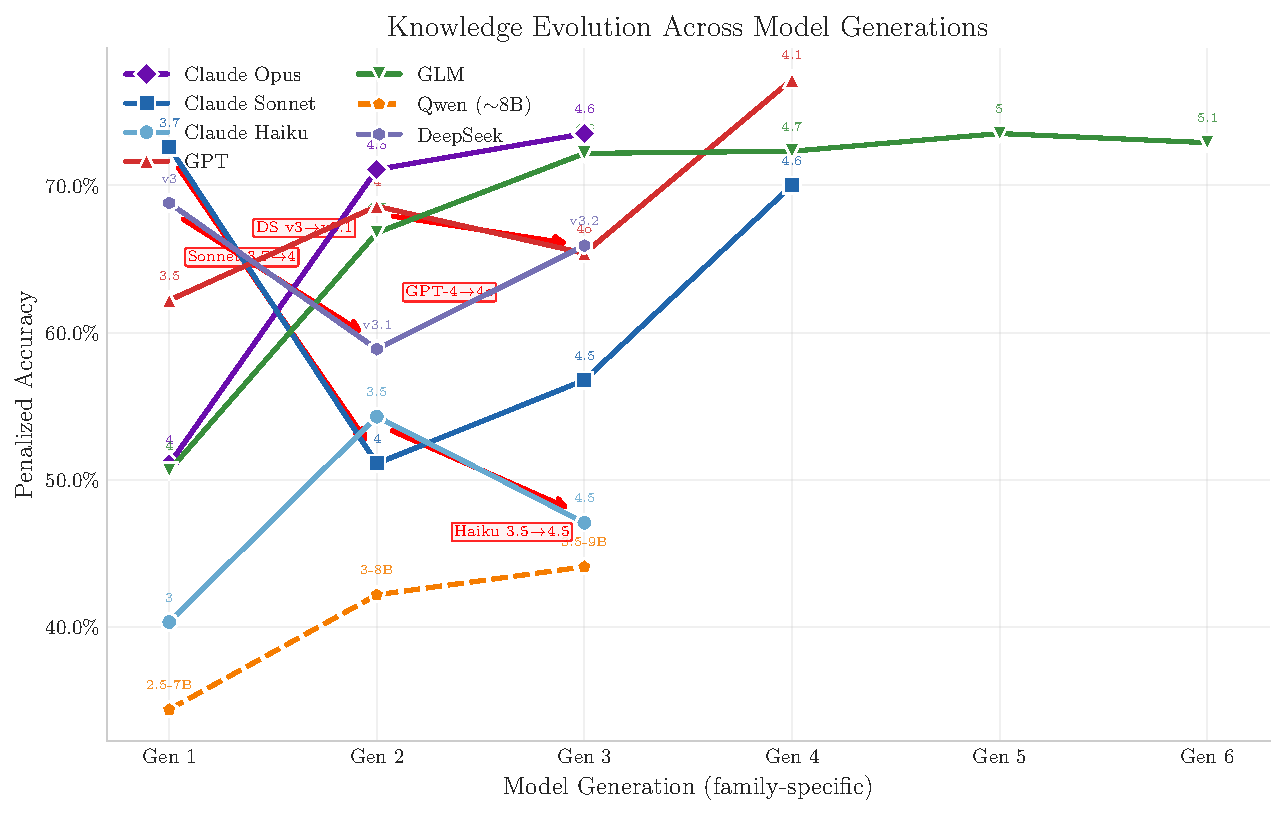
\includegraphics[width=\textwidth]{figures/fig_a3_generation_trajectories.pdf}
    \caption{Knowledge evolution across model generations. Red boxes highlight regressions: GPT-4$\to$4o (smaller efficiency-optimized successor), Claude Sonnet 3.7$\to$4 (RLHF conservatism), Claude Haiku 3.5$\to$4.5 (smaller post-training). GLM shows the steadiest improvement across 6 generations.}
    \label{fig:gen-trajectories}
\end{figure}

\begin{figure}[H]
    \centering
    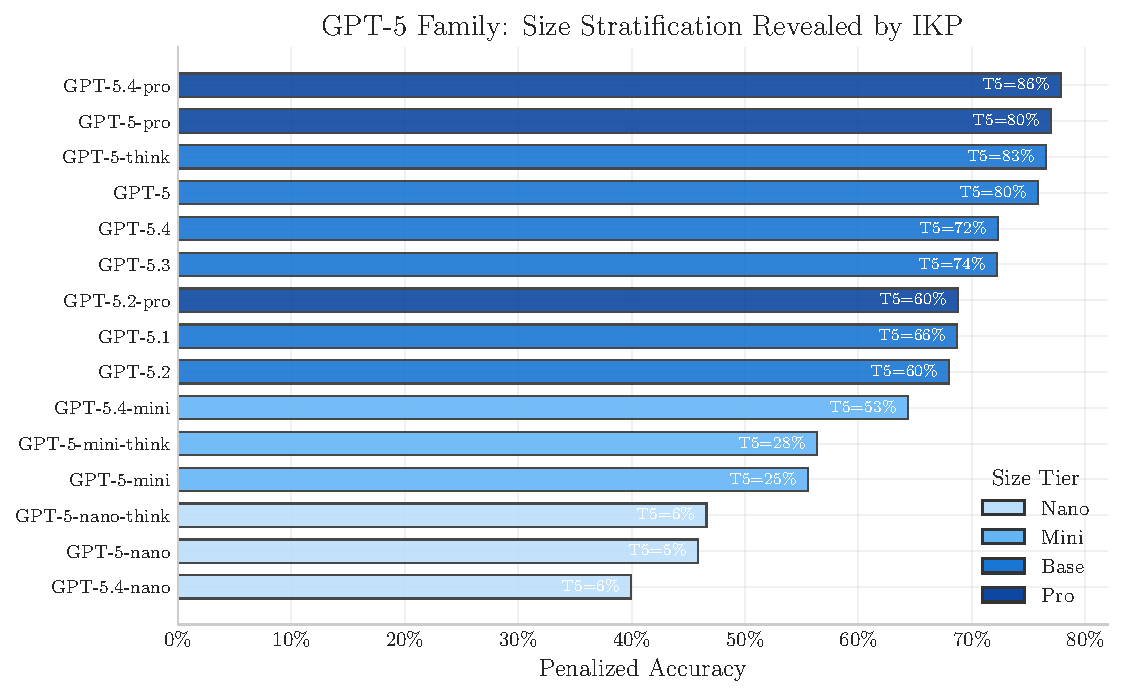
\includegraphics[width=0.9\textwidth]{figures/fig_a4_gpt5_family.pdf}
    \caption{GPT-5 family size stratification revealed by IKP. T5 accuracy (annotated) shows clear tiers: nano (0--3\%), mini (19--41\%), base (51--77\%), pro (74--76\%). GPT-5, GPT-5-pro, and GPT-5-think score nearly identically, suggesting the same base model with different inference configurations.}
    \label{fig:gpt5-family}
\end{figure}

\section{Knowledge Fingerprinting: Detailed Tables}
\label{app:fingerprint}

This appendix expands Section~\ref{sec:fingerprint} with the complete consecutive-pair tables for each tracked model family and the full list of cross-vendor outliers. For every pair of models we report, on the 400 T5--T6 probes, the Jaccard similarity $J$ of correct-answer sets, the lift ($= \text{observed}/\text{expected}$, under the null of independence) of the correct-set intersection, the hallucination similarity $\mathrm{HSS}$, the number of joint-wrong probes (``both\_w''), and a regime classification (shared-base, lineage, retrained, independent). The thresholds are those stated in Section~\ref{sec:fingerprint}: shared-base requires $\mathrm{HSS} \geq 0.30$ and $J \geq 0.60$; lineage requires $\mathrm{HSS} \geq 0.10$ and $J \geq 0.50$; retrained is $\mathrm{HSS} < 0.10$ with $\geq 10$ joint-wrong probes (limited statistical resolution when both\_w is much smaller).

\paragraph{Why HSS?} Raw Jaccard on correct-answer sets is dominated by probes that nearly all frontier models get right, producing high $J$ even for truly independent models (for example, GPT-5 vs.\ Claude Opus 4.5 scores $J = 0.56$ despite being independent trainings by different vendors). Lift partially corrects for this but is noisy when either model's correct set is small. Hallucination similarity---the rate at which two models produce the same normalized wrong answer on a probe that both got wrong---is a much cleaner signal: independent models almost never converge on the same wrong rare fact, while weight-sharing siblings do so on 30--55\% of joint-wrong probes. A bright threshold around $\mathrm{HSS} = 0.30$ separates the two regimes empirically.

\paragraph{When the three metrics disagree.} The three metrics are complementary, not redundant. Heavy post-training can preserve rare-fact knowledge (high $J$ and high lift) while rewriting the generation style enough that a model gives \emph{differently worded} wrong answers on hard probes---driving $\mathrm{HSS}$ down. Nemotron-70B vs.\ Llama-3.1-70B is the textbook example: $J = 0.79$ and lift = 7.5 (clear shared base) but $\mathrm{HSS} = 0.08$ (SFT has scrambled the surface form of wrong answers). Conversely, a high-$\mathrm{HSS}$ pair with low $J$ and low lift is a weaker signal than it sounds, because it may reflect a single over-represented hallucination (e.g., a common name collision) rather than broad knowledge overlap. We classify a pair as \emph{shared base} only when all three metrics point the same way; one-sided signals are reported as ``possible lineage'' and should be investigated case-by-case.

\paragraph{Release-practice summary.} Applied to consecutive-generation pairs across all tracked families (see Table~\ref{tab:fp-all-families}), three release patterns recur:
\begin{itemize}[leftmargin=*]
    \item \emph{Fine-tune-on-same-base releases} (lineage): Claude Opus 4 $\to$ 4.1, Sonnet 4 $\to$ 4.5, DeepSeek V3 $\to$ V3.1 $\to$ V3.2, GLM 4.6 $\to$ 4.7, Kimi K2 $\to$ K2.5 $\to$ K2.6. These preserve a large fraction of the base's rare-fact mistakes.
    \item \emph{Inference/alignment variants of a shared base} (shared-base): GPT-5 / GPT-5-pro / GPT-5-think; GPT-5.2 / 5.2-pro; Claude Opus 4.5 / 4.5-think. These show the highest $\mathrm{HSS}$ in the dataset.
    \item \emph{Full retrains} (retrained): every GPT-5.$x$ $\to$ 5.$(x{+}1)$ transition for $x = 0,1,2,3$; Claude Opus 4.6 $\to$ 4.7; every cross-generation Gemini pair; GLM 4.7 $\to$ 5 and 5 $\to$ 5.1. For these, the same-wrong-answer count is statistically indistinguishable from what we see between models built by different vendors, despite the shared version-family label.
\end{itemize}

\paragraph{Cross-vendor outliers: how to read the table.} Applying the same test to the ${\sim}13\,000$ cross-vendor pairs flags a small fraction at $\mathrm{HSS} \geq 0.20$ with $\geq 10$ joint-wrong probes (the full list is Table~\ref{tab:fp-cross-full}). Interpretation requires care: a single high-$\mathrm{HSS}$ pair between two independent frontier models is not strong evidence of cross-family distillation given the number of pairs tested. More suggestive is the \emph{pattern} across pairs involving the same model on one side:

\begin{itemize}[leftmargin=*]
    \item \textbf{Baidu ERNIE 4.5-300B-A47B} is above the cross-vendor threshold against five independent models simultaneously (GPT-4o $\mathrm{HSS}=0.44$, Llama-3-70B $0.43$, Mistral-Large $0.40$, Qwen-Max $0.33$, Mistral-Small-24B $0.33$). This is the pattern expected when a model is trained on a large mixture of distilled outputs from Western frontier models rather than on a single teacher.
    \item \textbf{Llama 3.1 70B} appears as an apparent ``teacher'' against many other models ($\mathrm{HSS} \geq 0.30$ vs.\ grok-3, gemini-2.0-flash, qwen3-max, nova-pro, and several older OpenAI models). This is consistent with Llama 3.1 being the most widely-used open base for synthetic-data generation in 2024--2025, so its characteristic hallucinations leak into many downstream datasets. It is \emph{not} evidence that any single downstream vendor distilled from it directly.
    \item \textbf{deepseek-r1-distill-llama-70b vs.\ Llama-3.1-70B} ($\mathrm{HSS} = 0.33$) is a known distillation-into-base pairing and serves as a positive control for the method.
    \item Individual high-$\mathrm{HSS}$ frontier-vs-frontier pairs (GPT-5 vs.\ Grok-4 at $0.31$; GPT-5-pro vs.\ Kimi-K2.6 at $0.27$) are individually above threshold but have too few joint-wrong probes, at our probe count, to reject an innocent-explanation null (e.g., training on similar recent web snapshots or on overlapping synthetic-data mixtures).
\end{itemize}

\paragraph{Limitations.} The method identifies \emph{statistical} overlap in knowledge and hallucination patterns; it does not distinguish between direct distillation and shared training data (e.g., two vendors independently scraping the same recent Wikipedia dump or licensing the same curated corpus). It also has limited resolution when the number of joint-wrong rare-fact probes is small: frontier models that each score 70--80\% on T5--T6 jointly get only 20--50 probes wrong, and $\mathrm{HSS}$ estimated from small samples is noisy. Probe-pool expansion into T6--T7 would tighten these estimates and is a natural next step.

\paragraph{Known-provenance positive controls.} As a sanity check, Table~\ref{tab:fp-controls} reports metrics for six pairs whose parent-child relationship is publicly disclosed. Every pair with $\geq 10$ joint-wrong probes shows elevated lift (2.4--7.5) and $J$ (0.32--0.79) consistent with shared training signal; $\mathrm{HSS}$ on heavily post-trained derivatives (Nemotron, R1-distill) is suppressed for the reason discussed above, which is why we recommend using all three metrics jointly rather than thresholding $\mathrm{HSS}$ alone.

% auto-generated by scripts/14_comprehensive_fingerprinting.py
\begin{table}[ht]\centering\small
\begin{tabular}{p{0.30\textwidth} p{0.22\textwidth} r r r r}
\toprule Student (derived) & Parent (base/teacher) & $J$ & lift & HSS & both\_w \\ \midrule
deepseek-r1-distill-llama-70b-think & llama-3.3-70b & 0.315 & 2.39 & 0.125 & 32 \\
deepseek-r1-distill-qwen-32b-think & qwq-32b-think & 0.317 & 7.39 & 0.038 & 182 \\
nemotron-70b & llama-3.1-70b & 0.792 & 7.47 & 0.077 & 13 \\
nemotron-super-49b-think & llama-3.3-70b & 0.167 & 2.36 & 0.069 & 29 \\
hermes-3-405b & llama-3.1-70b & 0.255 & 7.62 & 1.000 & 2 \\
hermes-4-405b & hermes-3-405b & 0.275 & 8.49 & 1.000 & 3 \\
\bottomrule \end{tabular}
\caption{Known-provenance positive controls. Each pair is a publicly-disclosed distillation or fine-tune. All show either lineage or cross-vendor-suspect HSS ($\geq 0.10$) when both\_w permits statistical resolution, confirming that the HSS metric detects shared training signal.}\label{tab:fp-controls}\end{table}

\paragraph{Comprehensive all-family table.} Table~\ref{tab:fp-all-families} reports consecutive-generation metrics for every tracked family (open-weight and closed-weight) where at least one consecutive pair has $\geq 8$ joint-wrong probes. Three patterns recur across the ${\sim}30$ families:
\begin{itemize}[leftmargin=*]
    \item \emph{Frequent retrains}: Gemini Flash/Pro, Gemma 2/3/4, Qwen 2.5/3/3.5, most GPT-5 \texttt{.x} transitions, and the Opus 4.6/4.7 step all sit in the retrained regime. These vendors appear to prefer full retrains over incremental post-training when bumping version numbers.
    \item \emph{Incremental lineages}: DeepSeek V3 $\to$ V3.1 $\to$ V3.2, GLM 4.6 $\to$ 4.7, Kimi K2 $\to$ K2.5 $\to$ K2.6, and the Nova / Command families show consistent lineage-regime HSS, consistent with continued pretraining or large-scale post-training on a stable base.
    \item \emph{Shared-base variants}: Thinking / reasoning variants (Opus 4.5 / 4.5-think, GPT-5.2 / 5.2-pro, DeepSeek V3.2 / V3.2-think) and ``pro'' variants of the same base generation concentrate at $\mathrm{HSS} \geq 0.30$.
\end{itemize}

% auto-generated by scripts/14_comprehensive_fingerprinting.py
{\small
\begin{longtable}{@{}p{0.20\textwidth} p{0.20\textwidth} r r r r l@{}}
\caption{Comprehensive within-family fingerprint metrics for all tracked model families (T5--T6 probes). $J$: Jaccard on correct-answer sets; lift: observed/expected-under-independence; $\mathrm{HSS}$: hallucination similarity; both\_w: joint-wrong probes; class: shared-base / lineage / retrained / independent. Families with all pairs having both\_w $<$ 8 are omitted.}\label{tab:fp-all-families}\\
\toprule From & To & $J$ & lift & HSS & both\_w & class \\ \midrule \endfirsthead
\toprule From & To & $J$ & lift & HSS & both\_w & class \\ \midrule \endhead
\multicolumn{7}{l}{\emph{OpenAI GPT base}} \\
\quad gpt-3.5-turbo & gpt-4 & 0.448 & 1.72 & 0.078 & 51 & retrained \\
\quad gpt-4 & gpt-4-turbo & 0.647 & 1.59 & 0.089 & 45 & retrained \\
\quad gpt-4-turbo & gpt-4o & 0.482 & 1.47 & 0.200 & 30 & independent \\
\quad gpt-4o & gpt-4.1 & 0.538 & 1.46 & 0.318 & 22 & lineage \\
\quad gpt-4.1 & gpt-5 & 0.758 & 1.38 & 0.000 & 38 & retrained \\
\quad gpt-5 & gpt-5.1 & 0.656 & 1.53 & 0.000 & 22 & retrained \\
\quad gpt-5.1 & gpt-5.2 & 0.555 & 1.69 & 0.091 & 11 & retrained \\
\quad gpt-5.2 & gpt-5.3 & 0.596 & 1.67 & 0.000 & 23 & retrained \\
\quad gpt-5.3 & gpt-5.4 & 0.715 & 1.63 & 0.083 & 48 & retrained \\
\multicolumn{7}{l}{\emph{OpenAI GPT-5 base/pro/think cluster}} \\
\quad gpt-5 & gpt-5-pro & 0.836 & 1.48 & 0.561 & 41 & shared-base \\
\quad gpt-5-pro & gpt-5-think & 0.846 & 1.46 & 0.523 & 44 & shared-base \\
\multicolumn{7}{l}{\emph{OpenAI GPT-5 .x transitions}} \\
\quad gpt-5 & gpt-5.1 & 0.656 & 1.53 & 0.000 & 22 & retrained \\
\quad gpt-5.1 & gpt-5.2 & 0.555 & 1.69 & 0.091 & 11 & retrained \\
\quad gpt-5.2 & gpt-5.2-pro & 0.776 & 2.15 & 0.286 & 42 & lineage \\
\quad gpt-5.2-pro & gpt-5.3 & 0.597 & 1.64 & 0.038 & 26 & retrained \\
\quad gpt-5.3 & gpt-5.4 & 0.715 & 1.63 & 0.083 & 48 & retrained \\
\quad gpt-5.4 & gpt-5.4-pro & 0.715 & 1.44 & 0.101 & 69 & lineage \\
\multicolumn{7}{l}{\emph{OpenAI GPT-mini}} \\
\quad gpt-4o-mini & gpt-4.1-mini & 0.304 & 2.06 & 0.070 & 143 & retrained \\
\quad gpt-4.1-mini & gpt-5-mini & 0.361 & 2.45 & 0.286 & 7 & independent \\
\quad gpt-5-mini & gpt-5.4-mini & 0.311 & 2.27 & 0.000 & 5 & independent \\
\multicolumn{7}{l}{\emph{OpenAI GPT-nano}} \\
\quad gpt-4.1-nano & gpt-5-nano & 0.107 & 4.38 & 0.000 & 8 & independent \\
\quad gpt-5-nano & gpt-5.4-nano & 0.100 & 6.67 & 0.000 & 4 & independent (small $n$) \\
\multicolumn{7}{l}{\emph{OpenAI o-series}} \\
\quad o1 & o3-mini & 0.131 & 1.62 & 0.000 & 17 & retrained \\
\quad o3-mini & o3 & 0.120 & 1.47 & 0.000 & 29 & retrained \\
\quad o3 & o4-mini-think & 0.404 & 1.38 & 0.000 & 46 & retrained \\
\multicolumn{7}{l}{\emph{Anthropic Claude Opus}} \\
\quad claude-opus-4 & claude-opus-4.1 & 0.525 & 6.56 & 0.889 & 9 & lineage \\
\quad claude-opus-4.1 & claude-opus-4.5 & 0.282 & 1.87 & 0.111 & 9 & independent \\
\quad claude-opus-4.5 & claude-opus-4.6 & 0.757 & 1.62 & 0.091 & 33 & retrained \\
\quad claude-opus-4.6 & claude-opus-4.7 & 0.604 & 1.64 & 0.000 & 15 & retrained \\
\multicolumn{7}{l}{\emph{Anthropic Claude Sonnet}} \\
\quad claude-3.7-sonnet & claude-sonnet-4 & 0.141 & 1.72 & 0.250 & 4 & independent (small $n$) \\
\quad claude-sonnet-4 & claude-sonnet-4.5 & 0.449 & 5.61 & 0.429 & 7 & independent \\
\quad claude-sonnet-4.5 & claude-sonnet-4.6 & 0.324 & 2.00 & 0.133 & 15 & independent \\
\multicolumn{7}{l}{\emph{Anthropic Claude Haiku}} \\
\quad claude-3-haiku & claude-3.5-haiku & 0.041 & 2.82 & 0.000 & 1 & independent (small $n$) \\
\quad claude-3.5-haiku & claude-haiku-4.5 & 0.136 & 2.95 & 0.167 & 18 & independent \\
\multicolumn{7}{l}{\emph{Google Gemini Flash}} \\
\quad gemini-2.0-flash & gemini-2.5-flash & 0.497 & 2.14 & 0.021 & 48 & retrained \\
\quad gemini-2.5-flash & gemini-3-flash & 0.297 & 1.09 & 0.067 & 15 & retrained \\
\multicolumn{7}{l}{\emph{Google Gemini Flash-Lite}} \\
\quad gemini-2.5-flash-lite & gemini-3.1-flash-lite & 0.237 & 1.29 & 0.029 & 70 & retrained \\
\multicolumn{7}{l}{\emph{Google Gemma}} \\
\quad gemma-2-2b & gemma-3-1b & 0.048 & 4.10 & 0.014 & 284 & retrained \\
\quad gemma-3-1b & gemma-3-4b & 0.000 & 0.00 & 0.006 & 349 & retrained \\
\quad gemma-3-4b & gemma-3-12b & 0.200 & 6.48 & 0.042 & 334 & retrained \\
\quad gemma-3-12b & gemma-2-27b & 0.000 & 0.00 & 0.044 & 90 & retrained \\
\quad gemma-2-27b & gemma-3-27b & 0.118 & 3.81 & 0.047 & 85 & retrained \\
\quad gemma-3-27b & gemma-4-31b & 0.076 & 1.33 & 0.000 & 238 & retrained \\
\multicolumn{7}{l}{\emph{Meta Llama 3 (70B)}} \\
\quad llama-3-70b & llama-3.1-70b & 0.424 & 4.06 & 0.625 & 8 & independent \\
\quad llama-3.1-70b & llama-3.3-70b & 0.500 & 4.42 & 0.400 & 15 & lineage \\
\multicolumn{7}{l}{\emph{Meta Llama 3 (8B)}} \\
\quad llama-3-8b & llama-3.1-8b & 0.214 & 12.70 & 0.125 & 8 & independent \\
\multicolumn{7}{l}{\emph{Meta Llama 4}} \\
\quad llama-4-scout & llama-4-maverick & 0.255 & 2.01 & 0.065 & 46 & retrained \\
\multicolumn{7}{l}{\emph{Alibaba Qwen dense (7B)}} \\
\quad qwen-2.5-7b & qwen3-8b-think & 0.143 & 10.26 & 0.040 & 100 & retrained \\
\multicolumn{7}{l}{\emph{Alibaba Qwen dense (70B)}} \\
\quad qwen-2.5-72b & qwq-32b-think & 0.218 & 4.28 & 0.032 & 62 & retrained \\
\multicolumn{7}{l}{\emph{Alibaba Qwen Max}} \\
\quad qwen-max & qwen3-max & 0.224 & 2.34 & 0.231 & 13 & independent \\
\multicolumn{7}{l}{\emph{Alibaba Qwen Plus}} \\
\quad qwen-plus & qwen3.5-plus-think & 0.464 & 2.10 & 0.000 & 94 & retrained \\
\quad qwen3.5-plus-think & qwen3.6-plus-think & 0.545 & 2.36 & 0.105 & 19 & lineage \\
\multicolumn{7}{l}{\emph{Alibaba Qwen large MoE}} \\
\quad qwen3-235b-a22b-think & qwen3.5-397b-a17b-think & 0.243 & 2.40 & 0.011 & 87 & retrained \\
\multicolumn{7}{l}{\emph{DeepSeek V3}} \\
\quad deepseek-v3 & deepseek-v3.1 & 0.380 & 1.82 & 0.227 & 22 & independent \\
\quad deepseek-v3.1 & deepseek-v3.2 & 0.503 & 2.25 & 0.333 & 21 & lineage \\
\multicolumn{7}{l}{\emph{Zhipu GLM}} \\
\quad glm-4.5-think & glm-4.6-think & 0.572 & 1.66 & 0.041 & 49 & retrained \\
\quad glm-4.6-think & glm-4.7-think & 0.707 & 1.58 & 0.209 & 129 & lineage \\
\quad glm-4.7-think & glm-5-think & 0.561 & 1.33 & 0.011 & 92 & retrained \\
\quad glm-5-think & glm-5.1-think & 0.687 & 1.46 & 0.012 & 84 & retrained \\
\multicolumn{7}{l}{\emph{xAI Grok}} \\
\quad grok-3 & grok-4 & 0.779 & 1.45 & 0.027 & 37 & retrained \\
\quad grok-4 & grok-4.20 & 0.557 & 1.38 & 0.000 & 44 & retrained \\
\multicolumn{7}{l}{\emph{Moonshot Kimi K2}} \\
\quad kimi-k2 & kimi-k2.5-think & 0.574 & 1.48 & 0.023 & 44 & retrained \\
\quad kimi-k2.5-think & kimi-k2.6-think & 0.765 & 1.63 & 0.510 & 49 & shared-base \\
\multicolumn{7}{l}{\emph{Mistral large/medium}} \\
\quad mistral-medium-3.1 & mistral-large & 0.420 & 3.19 & 0.000 & 33 & retrained \\
\multicolumn{7}{l}{\emph{Mistral small/open}} \\
\quad mistral-7b & mistral-nemo-12b & 0.189 & 5.80 & 0.018 & 164 & retrained \\
\quad mistral-nemo-12b & mistral-small-24b & 0.324 & 8.03 & 0.066 & 61 & retrained \\
\multicolumn{7}{l}{\emph{Mistral MoE (Mixtral)}} \\
\quad mixtral-8x7b & mixtral-8x22b & 0.209 & 1.78 & 0.000 & 51 & retrained \\
\multicolumn{7}{l}{\emph{Mistral ministral}} \\
\quad ministral-3b & ministral-8b & 0.085 & 2.46 & 0.023 & 264 & retrained \\
\multicolumn{7}{l}{\emph{Amazon Nova}} \\
\quad nova-micro & nova-pro & 0.135 & 3.51 & 0.070 & 114 & retrained \\
\quad nova-pro & nova-premier & 0.327 & 2.24 & 0.008 & 122 & retrained \\
\multicolumn{7}{l}{\emph{Cohere Command}} \\
\quad command-r7b & command-r-plus & 0.026 & 1.30 & 0.000 & 27 & retrained \\
\quad command-r-plus & command-a & 0.232 & 3.50 & 0.053 & 19 & retrained \\
\multicolumn{7}{l}{\emph{Microsoft Phi}} \\
\quad phi-3-mini & phi-4 & 0.000 & 0.00 & 0.000 & 181 & retrained \\
\bottomrule
\end{longtable}
}

\paragraph{All cross-vendor outliers.} Table~\ref{tab:fp-cross-full} gives the full ranked list of cross-vendor pairs above our reporting threshold.

% auto-generated by scripts/14_comprehensive_fingerprinting.py
{\small
\begin{longtable}{p{0.30\textwidth} p{0.30\textwidth} r r r r}
\caption{Complete list of cross-vendor outlier pairs with $\mathrm{HSS} \geq 0.20$ and $\geq 10$ joint-wrong probes on T5--T6.}\label{tab:fp-cross-full} \\
\toprule Model A & Model B & $J$ & lift & HSS & both\_w \\ \midrule \endfirsthead
\toprule Model A & Model B & $J$ & lift & HSS & both\_w \\ \midrule \endhead
ernie-4.5-300b-a47b & llama-3-70b & 0.433 & 3.79 & 0.500 & 12 \\
gpt-4.1-nano & llama-3.1-70b & 0.160 & 1.86 & 0.467 & 15 \\
ernie-4.5-300b-a47b & gpt-4o & 0.302 & 2.21 & 0.462 & 13 \\
gemini-2.0-flash & llama-3.1-70b & 0.278 & 2.35 & 0.462 & 13 \\
claude-opus-4.7 & gpt-5 & 0.534 & 1.46 & 0.417 & 12 \\
claude-opus-4.7 & kimi-k2.6-think & 0.546 & 1.62 & 0.400 & 10 \\
ernie-4.5-300b-a47b & mistral-small-24b & 0.254 & 4.51 & 0.400 & 15 \\
gpt-3.5-turbo & hermes-4-405b & 0.252 & 2.60 & 0.400 & 10 \\
grok-3 & llama-3.1-70b & 0.147 & 1.24 & 0.400 & 10 \\
llama-3-70b & mistral-large & 0.512 & 4.20 & 0.385 & 13 \\
gpt-5 & grok-4 & 0.587 & 1.23 & 0.381 & 21 \\
claude-opus-4.7 & gpt-5-think & 0.524 & 1.42 & 0.364 & 11 \\
gpt-4o-mini & hermes-4-405b & 0.262 & 3.27 & 0.364 & 11 \\
grok-3 & qwen-max & 0.145 & 1.50 & 0.364 & 11 \\
llama-3.1-70b & qwen3-max & 0.202 & 1.77 & 0.364 & 11 \\
llama-4-maverick & qwen-max & 0.209 & 2.25 & 0.364 & 11 \\
ernie-4.5-300b-a47b & qwen-max & 0.293 & 3.89 & 0.357 & 14 \\
gpt-5.5-pro & kimi-k2.6-think & 0.556 & 1.16 & 0.357 & 14 \\
claude-opus-4.8 & deepseek-v4-flash & 0.314 & 1.33 & 0.353 & 17 \\
gemini-2.5-flash & gpt-5-pro & 0.365 & 1.40 & 0.353 & 17 \\
claude-opus-4.7-think & llama-3-70b & 0.350 & 2.05 & 0.333 & 12 \\
gpt-5 & kimi-k2.6-think & 0.573 & 1.33 & 0.333 & 21 \\
gpt-5-pro & kimi-k2.6-think & 0.582 & 1.34 & 0.318 & 22 \\
deepseek-r1-distill-llama-70b-think & llama-3.1-70b & 0.220 & 2.16 & 0.312 & 16 \\
claude-opus-4.7-think & deepseek-v4-flash & 0.525 & 1.35 & 0.308 & 26 \\
claude-opus-4.8 & hy3-preview & 0.310 & 1.33 & 0.308 & 13 \\
gpt-4 & llama-3.1-70b & 0.241 & 1.97 & 0.308 & 13 \\
gpt-4o & kimi-k2 & 0.379 & 1.36 & 0.308 & 13 \\
claude-opus-4.7 & ernie-4.5-300b-a47b & 0.295 & 2.15 & 0.300 & 10 \\
claude-opus-4.8 & gemini-3.1-flash-lite & 0.319 & 1.30 & 0.300 & 10 \\
claude-sonnet-4.5 & gemini-3.1-flash-lite & 0.227 & 1.37 & 0.300 & 10 \\
claude-sonnet-4.5 & gpt-4.1 & 0.247 & 1.49 & 0.300 & 10 \\
claude-sonnet-4.5 & gpt-4o & 0.310 & 2.03 & 0.300 & 10 \\
claude-sonnet-4.5 & kimi-k2 & 0.280 & 1.82 & 0.300 & 10 \\
deepseek-v4-pro & gemini-3.1-flash-lite & 0.262 & 1.26 & 0.300 & 10 \\
gemini-3.1-flash-lite & llama-3.1-70b & 0.161 & 1.31 & 0.300 & 10 \\
hermes-4-405b & qwen3-next-80b-a3b & 0.293 & 3.81 & 0.300 & 10 \\
kimi-k2 & llama-3.1-70b & 0.208 & 1.78 & 0.300 & 10 \\
mistral-large & qwen-max & 0.420 & 5.04 & 0.300 & 10 \\
gpt-4o & llama-4-maverick & 0.459 & 1.68 & 0.294 & 17 \\
claude-sonnet-4.5-think & gpt-4o & 0.417 & 1.62 & 0.286 & 14 \\
deepseek-v4-flash & mistral-large & 0.211 & 1.47 & 0.286 & 14 \\
deepseek-v4-pro & gpt-4o-mini & 0.238 & 2.08 & 0.286 & 14 \\
gpt-4.1 & grok-3-mini-think & 0.350 & 1.45 & 0.286 & 14 \\
kimi-k2 & mistral-large & 0.285 & 2.02 & 0.286 & 21 \\
gemini-2.5-flash & gpt-5-think & 0.370 & 1.41 & 0.278 & 18 \\
claude-haiku-4.5 & gpt-4.1 & 0.069 & 1.34 & 0.273 & 11 \\
claude-opus-4.8 & kimi-k2 & 0.319 & 1.51 & 0.273 & 11 \\
command-r-plus & grok-4 & 0.105 & 1.51 & 0.273 & 11 \\
deepseek-v4-pro & gpt-4.1 & 0.294 & 1.40 & 0.273 & 11 \\
deepseek-v4-pro & o4-mini-think & 0.329 & 1.94 & 0.273 & 11 \\
gemini-3-flash & grok-3-mini-think & 0.277 & 1.12 & 0.273 & 11 \\
glm-4.5-air-think & gpt-5-mini-think & 0.339 & 2.69 & 0.273 & 11 \\
gpt-4.1-nano & hermes-4-405b & 0.150 & 1.96 & 0.273 & 11 \\
gpt-5-think & mistral-small-24b & 0.090 & 1.40 & 0.273 & 11 \\
grok-3 & mistral-large & 0.210 & 1.46 & 0.273 & 11 \\
llama-3.1-70b & nova-pro & 0.258 & 2.87 & 0.273 & 11 \\
claude-opus-4.8 & gemini-2.0-flash & 0.441 & 2.06 & 0.267 & 15 \\
gpt-4o & qwen3-max & 0.420 & 1.52 & 0.261 & 23 \\
kimi-k2.6-think & o3 & 0.573 & 1.31 & 0.261 & 23 \\
glm-5-turbo-think & grok-4 & 0.592 & 1.42 & 0.258 & 31 \\
claude-opus-4.7 & gemini-2.5-flash & 0.428 & 1.85 & 0.250 & 12 \\
claude-opus-4.7 & mixtral-8x22b & 0.373 & 1.81 & 0.250 & 12 \\
claude-opus-4.7 & o3 & 0.496 & 1.36 & 0.250 & 12 \\
claude-opus-4.7-think & qwen3.7-max & 0.552 & 1.53 & 0.250 & 16 \\
claude-opus-4.8 & glm-4.5-air-think & 0.348 & 2.18 & 0.250 & 12 \\
claude-opus-4.8 & grok-3-mini-think & 0.358 & 2.10 & 0.250 & 12 \\
claude-sonnet-4.5 & gpt-4 & 0.303 & 1.88 & 0.250 & 12 \\
deepseek-v4-flash & qwen-max & 0.145 & 1.51 & 0.250 & 16 \\
deepseek-v4-pro & qwen3-next-80b-a3b & 0.291 & 2.68 & 0.250 & 16 \\
ernie-4.5-300b-a47b & grok-3 & 0.197 & 1.40 & 0.250 & 20 \\
ernie-4.5-300b-a47b & llama-4-maverick & 0.244 & 1.89 & 0.250 & 20 \\
gemini-2.0-flash & qwen-max & 0.190 & 2.08 & 0.250 & 16 \\
gpt-5.5-think & kimi-k2.6-think & 0.546 & 1.16 & 0.250 & 16 \\
grok-3 & llama-3-70b & 0.258 & 1.49 & 0.250 & 16 \\
llama-3-70b & mistral-small-24b & 0.228 & 3.90 & 0.250 & 12 \\
glm-5-turbo-think & gpt-5 & 0.550 & 1.33 & 0.241 & 29 \\
gemini-2.0-flash & gpt-4o & 0.487 & 1.77 & 0.240 & 25 \\
gemini-2.5-pro & grok-4 & 0.550 & 1.12 & 0.240 & 25 \\
gpt-4o & grok-3 & 0.400 & 1.21 & 0.238 & 21 \\
gpt-5.3 & grok-4 & 0.522 & 1.25 & 0.238 & 21 \\
claude-opus-4.7 & deepseek-v4-flash & 0.473 & 1.34 & 0.235 & 17 \\
gemini-2.5-flash & gpt-5 & 0.371 & 1.42 & 0.235 & 17 \\
gpt-5.5 & grok-4 & 0.618 & 1.12 & 0.235 & 17 \\
kimi-k2 & llama-3-70b & 0.322 & 1.94 & 0.235 & 17 \\
grok-3 & qwen3-max & 0.530 & 1.44 & 0.232 & 56 \\
claude-haiku-4.5 & ernie-4.5-300b-a47b & 0.162 & 3.61 & 0.231 & 13 \\
claude-haiku-4.5-think & deepseek-v3.2 & 0.190 & 2.29 & 0.231 & 13 \\
claude-opus-4.7 & gemini-2.5-pro-think & 0.498 & 1.34 & 0.231 & 13 \\
deepseek-r1-distill-llama-70b-think & llama-3-70b & 0.326 & 2.37 & 0.231 & 26 \\
gemma-2-27b & gpt-5 & 0.053 & 1.41 & 0.231 & 13 \\
gpt-3.5-turbo & llama-3.1-70b & 0.325 & 2.80 & 0.231 & 13 \\
ling-2.6-flash & seed-1.6-think & 0.151 & 3.22 & 0.231 & 13 \\
llama-3-70b & qwen-max & 0.358 & 4.19 & 0.231 & 13 \\
gemini-3.1-flash-lite & gpt-4o & 0.438 & 1.24 & 0.227 & 22 \\
gpt-5-think & grok-4 & 0.635 & 1.27 & 0.227 & 22 \\
claude-haiku-4.5 & deepseek-v3.2 & 0.122 & 2.35 & 0.222 & 18 \\
claude-opus-4.7 & gemini-2.5-flash-think & 0.515 & 1.57 & 0.222 & 18 \\
claude-opus-4.7 & glm-5 & 0.484 & 1.41 & 0.222 & 18 \\
claude-opus-4.8 & gpt-4o-mini & 0.350 & 2.63 & 0.222 & 18 \\
command-a & deepseek-v4-flash & 0.289 & 1.32 & 0.222 & 36 \\
gemini-2.5-pro-think & kimi-k2.6-think & 0.551 & 1.25 & 0.222 & 27 \\
glm-5.1 & gpt-5 & 0.566 & 1.29 & 0.222 & 36 \\
gpt-4 & llama-3.3-70b & 0.342 & 1.89 & 0.222 & 18 \\
deepseek-v4-flash & gemini-3-flash-think & 0.648 & 1.08 & 0.217 & 23 \\
claude-opus-4.8 & nova-pro & 0.280 & 2.17 & 0.214 & 14 \\
claude-sonnet-4.5 & glm-5-think & 0.265 & 1.63 & 0.214 & 14 \\
claude-sonnet-4.5-think & qwen-max & 0.254 & 2.66 & 0.214 & 14 \\
claude-sonnet-4.6 & deepseek-v3.1 & 0.361 & 1.68 & 0.214 & 14 \\
deepseek-v4-pro & gpt-3.5-turbo & 0.316 & 1.93 & 0.214 & 14 \\
gpt-4-turbo & qwen-max & 0.186 & 1.90 & 0.214 & 14 \\
gpt-4.1 & llama-3.3-70b & 0.267 & 1.44 & 0.214 & 14 \\
gpt-4.1-nano & llama-3-70b & 0.252 & 2.24 & 0.214 & 28 \\
gpt-4o & llama-3.3-70b & 0.371 & 2.13 & 0.214 & 14 \\
grok-3 & o1 & 0.543 & 1.22 & 0.214 & 14 \\
llama-4-maverick & mistral-large & 0.273 & 2.04 & 0.214 & 14 \\
mistral-small-24b & qwen-max & 0.204 & 4.34 & 0.214 & 14 \\
claude-sonnet-4.5-think & gemini-3.1-flash-lite & 0.439 & 1.32 & 0.211 & 19 \\
claude-sonnet-4.5-think & gpt-4 & 0.516 & 1.71 & 0.211 & 19 \\
gemini-2.0-flash & llama-3-70b & 0.338 & 2.13 & 0.208 & 24 \\
gpt-4o-mini & qwen-max & 0.241 & 3.21 & 0.208 & 24 \\
gpt-5-pro & grok-4 & 0.585 & 1.22 & 0.208 & 24 \\
gpt-5-think & kimi-k2.6-think & 0.601 & 1.36 & 0.208 & 24 \\
ernie-4.5-300b-a47b & glm-5.2 & 0.260 & 1.83 & 0.207 & 29 \\
gemini-2.5-flash & glm-5.1 & 0.356 & 1.47 & 0.207 & 29 \\
glm-5.1-think & gpt-5 & 0.576 & 1.25 & 0.207 & 29 \\
gpt-5 & kimi-k2.5-think & 0.564 & 1.21 & 0.205 & 44 \\
claude-3.5-haiku & ernie-4.5-300b-a47b & 0.217 & 2.23 & 0.200 & 10 \\
claude-3.5-haiku & hy3-preview & 0.253 & 1.48 & 0.200 & 10 \\
claude-3.5-haiku & kimi-k2 & 0.330 & 1.98 & 0.200 & 10 \\
claude-3.5-haiku & mistral-large & 0.226 & 2.29 & 0.200 & 10 \\
claude-haiku-4.5 & llama-3-70b & 0.165 & 3.49 & 0.200 & 10 \\
claude-haiku-4.5 & llama-4-maverick & 0.121 & 2.35 & 0.200 & 15 \\
claude-opus-4.7 & gpt-4o & 0.542 & 1.82 & 0.200 & 10 \\
claude-opus-4.7 & gpt-5.5-think & 0.453 & 1.18 & 0.200 & 10 \\
claude-opus-4.7 & qwen3-max & 0.529 & 1.76 & 0.200 & 15 \\
claude-opus-4.7 & qwen3.7-max & 0.524 & 1.57 & 0.200 & 10 \\
claude-sonnet-4-think & glm-5-think & 0.316 & 1.57 & 0.200 & 10 \\
claude-sonnet-4.5 & llama-4-maverick & 0.340 & 2.21 & 0.200 & 10 \\
claude-sonnet-4.5-think & llama-3.1-70b & 0.243 & 2.13 & 0.200 & 10 \\
command-a & gpt-4 & 0.351 & 1.66 & 0.200 & 20 \\
command-r-plus & glm-4.7-think & 0.112 & 1.63 & 0.200 & 15 \\
command-r-plus & seed-1.6-think & 0.198 & 3.12 & 0.200 & 25 \\
deepseek-r1-distill-llama-70b-think & hermes-4-405b & 0.214 & 2.38 & 0.200 & 10 \\
deepseek-v4-flash & llama-3.1-70b & 0.171 & 1.40 & 0.200 & 10 \\
deepseek-v4-pro & gemini-2.0-flash & 0.322 & 1.80 & 0.200 & 15 \\
deepseek-v4-pro & nemotron-3-ultra & 0.305 & 1.56 & 0.200 & 10 \\
gemini-2.5-flash & gpt-5.5 & 0.323 & 1.19 & 0.200 & 15 \\
gemini-2.5-flash & o3 & 0.366 & 1.39 & 0.200 & 25 \\
gemini-2.5-pro & gpt-5 & 0.632 & 1.20 & 0.200 & 25 \\
gemini-2.5-pro-think & gpt-5 & 0.635 & 1.21 & 0.200 & 25 \\
gemini-2.5-pro-think & grok-4 & 0.552 & 1.13 & 0.200 & 25 \\
gemma-3-270m & llama-3.3-70b & 0.041 & 0.51 & 0.200 & 10 \\
glm-4.5-air-think & llama-3.1-70b & 0.314 & 3.00 & 0.200 & 10 \\
glm-5.1-think & gpt-5-think & 0.592 & 1.25 & 0.200 & 30 \\
gpt-4 & qwen-max & 0.196 & 2.03 & 0.200 & 10 \\
gpt-4-turbo & llama-3.3-70b & 0.294 & 1.63 & 0.200 & 20 \\
gpt-5-mini-think & llama-4-maverick & 0.301 & 2.03 & 0.200 & 10 \\
grok-3-mini-think & mimo-v2-pro & 0.366 & 1.94 & 0.200 & 10 \\
hermes-4-405b & nemotron-3-super-120b & 0.185 & 2.09 & 0.200 & 10 \\
hy3-preview & mistral-large & 0.229 & 1.58 & 0.200 & 20 \\
ling-2.6-flash & qwen3.5-122b-a10b-think & 0.138 & 2.99 & 0.200 & 15 \\
llama-3.1-70b & nemotron-3-ultra & 0.211 & 1.76 & 0.200 & 10 \\
llama-3.1-70b & qwen3-235b-a22b-think & 0.119 & 1.82 & 0.200 & 10 \\
\bottomrule \end{longtable}
}

\section{Case Studies}
\label{app:case-studies}

This section presents concrete examples of probe questions and model responses to illustrate key findings from the main text. All responses are verbatim model outputs (truncated for space).

\subsection{USTC Hackergame --- Watching a Fact Arrive Over Three Years}
\label{app:hackergame-case}

The motivating observation in Section~\ref{sec:intro} traces the arrival of a single piece of long-tail knowledge---specific challenge names from \emph{USTC Hackergame}, an annual Capture-the-Flag competition organized by the USTC Linux User Group since 2014---into frontier model parameters across release cycles. We probed 12 representative models (across 2022--2026) with a uniform prompt asking for specific challenge names per year, then verified each response against the official writeup repositories at \url{https://github.com/USTC-Hackergame} and \url{https://github.com/ustclug/hackergame}. Results are summarized in Table~\ref{tab:hackergame-case}.

\paragraph{Three observations from this case study.}
\begin{enumerate}[leftmargin=*,topsep=2pt,itemsep=2pt]
    \item \textbf{The transition is sharp and dateable.} GPT-4o (May 2024) hallucinates a deterministic fake list, repeated across independent probes. Claude 3.7 Sonnet (February 2025) is the first model to list real per-year challenges, with $\sim$19 verified 2023 titles. Whatever change to the training pipeline absorbed Hackergame writeups happened in this $\sim$9-month window, not gradually across the field; later models (Claude Opus 4.6/4.7, GPT-5.5, Kimi K2.6) inherited and extended this knowledge.
    \item \textbf{Knowing the meta-fact does not imply knowing the content.} DeepSeek V4 Pro (1.6T) is the only model that correctly states 2014 as the start year (a single Wikipedia-grade meta-fact) but fabricates per-year challenges. The structural fact and the long-tail content are stored independently.
    \item \textbf{Refusal vs hallucination is a vendor-level choice that interacts with measurement.} GPT-4o and DeepSeek V4 Pro confidently fabricate; Claude Opus 4.7 says ``I don't have reliable detailed memory and don't want to fabricate specifics''; GPT-5/5.5 burn output budget on reasoning and produce empty content.
\end{enumerate}

This case is one motivating example among many; the systematic IKP probe set (Section~\ref{sec:probe-generation}) operationalizes the same kind of observation across 1{,}400 facts and 188 models, with quantitative scoring rather than human verification.

\begin{table}[H]
\centering
\small
\setlength{\tabcolsep}{4pt}
\begin{tabular}{l l p{10cm}}
\toprule
\textbf{Model} & \textbf{Released} & \textbf{Verification of LLM Responses} \\
\midrule
GPT-3.5 Turbo & 2022-11 & Hallucinates: claims contest started in ``2006'' (actual: 2014); claims ``offline finals'' (contest is online only). \\
GPT-4 & 2023-03 & Admits no specific knowledge. Generic CTF description. \\
GPT-4o & 2024-05 & Knows USTC + CTF format. Asked for per-year challenges, returns the \emph{identical} fabricated list (``Hello World'', ``Maze'', ``Calculator'', ``Reverse Engineering'', ``Quantum Computing'') for nine different years (2015--2023). None of these are real Hackergame challenges; the pattern is deterministic fabrication, repeated across two independent probes. \\
\textbf{Claude 3.7 Sonnet} & \textbf{2025-02} & \textbf{First model to list real per-year challenges.} 2023: ``Kitty Quiz'', ``Travel Photo'', ``Cyber Tic-Tac-Toe'', ``Committee Simulator'', ``High-Frequency Planet'', ``Streaming Planet'', ``Small LM Planet'', ``Word-Frugal'', ``Grandma's Bedtime flag Story'', ``Alien Detour'' (all verified real, English glosses of Chinese originals). Also accurate 2022 (HeiLang, Xcaptcha, plus original-Chinese titles) and 2021 (similar). \\
Gemini 2.5 Pro & 2025-03 & Lists $\sim$6 real challenges per year for 2021--2023 (e.g., HeiLang, ``JSON $\subset$ YAML?'', plus various original-Chinese titles), with one likely fabrication (a non-existent planet-series title). \\
GPT-5 & 2025-08 & Returns reasoning trace only; content cut off before any answer is written. \\
\textbf{Claude Opus 4.6} & \textbf{2025-11} & \textbf{Lists 16+ real Hackergame 2023 challenges, all verified}: ``Kitty Quiz'', ``Deeper Darker'', ``Travel Photo 3.0'', ``Cyber Tic-Tac-Toe'', ``Grandma's Bedtime flag Story'', ``Committee Simulator'', ``Worm'', ``JSON $\subset$ YAML?'', ``Git? Git!'', ``HTTP Stamp Album'', ``Docker for Everyone'', ``Word-Frugal 2.0'', ``High-Frequency Planet'', ``Streaming Planet'', ``Komm süsser satisfiability'', ``Alien Detour''. Earlier years also accurate. \\
Gemini 3.1 Pro & 2026-01 & Year-by-year breakdown 2018--2023 with specific real challenge names (``Travel Photo'', ``Selling Melons'', ``Transparent File'', ``Kitty Quiz'' series). Concise but accurate. \\
Kimi K2.6-think & 2026-03 & 30+ specific names across 2020--2023, mostly verified real (HeiLang, Xcaptcha, ``Cup-Window Goose-Shadow''/Wine, ``Komm süsser Flagge''), with occasional year-mixing. \\
DeepSeek V4 Pro & 2026-04 & Hallucinates: knows the meta-fact (correctly says contest started 2014, the only model that does) but fabricates per-year challenges as generic CTF tropes (``check-in problem'', ``classical cryptography'', ``web dog daily'', ``PWN intro'')---none are actual Hackergame names. \\
GPT-5.5 & 2026-04 & Lists real 2023 names (``Sign-In'', ``Kitty Quiz'', ``Deeper Darker'', ``Travel Photo 3.0'', ``JSON $\subset$ YAML?'', ``Git?'', ``HTTP Stamp Album'', ``Docker for Everyone'', ``Word-Frugal 2.0''). \\
Claude Opus 4.7 & 2026-04 & Year-by-year list 2018--2024. Specific names per year mostly real, with occasional cross-year mixing. Says contest started 2018 (incorrect: that was the year of the LUG renaming; contest itself dates to 2014). \\
\bottomrule
\end{tabular}
\caption{USTC Hackergame probe across 12 representative frontier models. Verification was performed against the official writeup repositories (\texttt{github.com/USTC-Hackergame/hackergame20\{18..23\}-writeups}) and the platform repo (\texttt{github.com/ustclug/hackergame}).}
\label{tab:hackergame-case}
\end{table}


\subsection{Tier Discrimination: Universal Knowledge (T1)}
\label{app:case-t1}

T1 probes test universal knowledge that every model, regardless of size, should know. Even the smallest 1B-parameter models answer these correctly.

\begin{quote}
\textbf{Probe:} What is the capital of France? \\
\textbf{Tier:} T1 \quad \textbf{Gold answer:} Paris \\
\textbf{Domain:} general \\
\end{quote}

\begin{description}[style=nextline, leftmargin=1.5cm]
\item[\textbf{Gemma-3 1B}] \textcolor{green!60!black}{\textsc{correct}} --- Paris.
\item[\textbf{Llama-3.2 3B}] \textcolor{green!60!black}{\textsc{correct}} --- Paris.
\item[\textbf{GPT-4o}] \textcolor{green!60!black}{\textsc{correct}} --- The capital of France is Paris.
\item[\textbf{Claude Opus 4.6}] \textcolor{green!60!black}{\textsc{correct}} --- Paris.
\end{description}

\subsection{Tier Discrimination: Mid-Tier Knowledge (T3)}
\label{app:case-t3}

T3 probes separate small models from medium and large ones. Small models ($<$10B) typically refuse or hallucinate, while models above ${\sim}30$B answer correctly. This probe tests a moderately obscure scientific fact.

\begin{quote}
\textbf{Probe:} Who first produced liquid helium? \\
\textbf{Tier:} T3 \quad \textbf{Gold answer:} Heike Kamerlingh Onnes \\
\textbf{Domain:} science \\
\end{quote}

\begin{description}[style=nextline, leftmargin=1.5cm]
\item[\textbf{Gemma-3 4B}] \textcolor{red!70!black}{\textsc{wrong}} --- William Ramsay and Lord Rayleigh.
\item[\textbf{Llama-3.2 3B}] \textcolor{orange!80!black}{\textsc{refusal}} --- I don't know.
\item[\textbf{GPT-4o}] \textcolor{green!60!black}{\textsc{correct}} --- Heike Kamerlingh Onnes first produced liquid helium in 1908.
\item[\textbf{Claude Opus 4.6}] \textcolor{green!60!black}{\textsc{correct}} --- Heike Kamerlingh Onnes first produced liquid helium on July 10, 1908, at his laboratory in Leiden, the Netherlands. This achievement earned him widespread recognition and contributed to his receiving the Nobel Prize in P...
\end{description}

\subsection{Tier Discrimination: Frontier-Only Knowledge (T6)}
\label{app:case-t6}

T6 probes are only answered correctly by the largest frontier models. These typically involve obscure researchers or rarely documented facts. Even strong models like GPT-4o refuse on these probes, while the top-scoring Gemini models retrieve the information.

\begin{quote}
\textbf{Probe:} In computer science, what is the research subfield of Janick Edinger, and name one paper, system, institution, or co-author associated with their work? If you don't know who this person is, say so. \\
\textbf{Tier:} T6 \quad \textbf{Gold answer:} distributed systems \\
\textbf{Domain:} computer\_science \\
\end{quote}

\begin{description}[style=nextline, leftmargin=1.5cm]
\item[\textbf{Llama-3.3 70B}] \textcolor{orange!80!black}{\textsc{refusal}} --- I don't know.
\item[\textbf{GPT-4o}] \textcolor{orange!80!black}{\textsc{refusal}} --- I don't know.
\item[\textbf{Gemini 3 Flash}] \textcolor{green!60!black}{\textsc{correct}} --- Janick Edinger's research subfield is distributed systems, with a specific focus on edge computing, pervasive computing, and mobile computing.
\item[\textbf{Gemini 3.1 Pro}] \textcolor{green!60!black}{\textsc{correct}} --- Janick Edinger's research subfields in computer science are primarily distributed systems, edge computing, pervasive/ubiquitous computing, and the Internet of Things (IoT).
\end{description}

\subsection{Hallucination vs.\ Refusal}
\label{app:case-hallucination}

A critical distinction in IKP evaluation is between hallucination (confidently wrong) and refusal (saying one does not know). Our scoring penalizes hallucination but not refusal, reflecting the real-world risk of confident misinformation. Here, Claude Opus 4.6 answers correctly, Llama-3.3 70B appropriately refuses, but GPT-4o-mini hallucinates a plausible but wrong subfield.

\begin{quote}
\textbf{Probe:} In computer science, what is the research subfield of Zhongzhi Luan, and name one paper, system, institution, or co-author associated with their work? If you don't know who this person is, say so. \\
\textbf{Tier:} T5 \quad \textbf{Gold answer:} computer architecture \\
\textbf{Domain:} computer\_science \\
\end{quote}

\begin{description}[style=nextline, leftmargin=1.5cm]
\item[\textbf{Claude Opus 4.6}] \textcolor{green!60!black}{\textsc{correct}} --- Zhongzhi Luan is a researcher in the field of high-performance computing (HPC). His research interests include parallel computing, large-scale cluster systems, and related areas in computer architecture and systems. He h...
\item[\textbf{Llama-3.3 70B}] \textcolor{orange!80!black}{\textsc{refusal}} --- I don't know.
\item[\textbf{GPT-4o-mini}] \textcolor{red!70!black}{\textsc{wrong}} --- Zhongzhi Luan is known for his research in the field of artificial intelligence, particularly in areas related to machine learning, data mining, and complex networks.
\end{description}

\subsection{Name Collision in Researcher Probes}
\label{app:case-name-collision}

Researcher probes are particularly susceptible to name collision: the model recognizes the name but associates it with a different person in the same or a different field. Here, ``Geoffrey Ye Li'' is a wireless communications researcher, but GPT-4o-mini confuses him with Geoffrey Hinton-adjacent ML researchers, producing a confident but wrong answer about ``deep learning and reinforcement learning.''

\begin{quote}
\textbf{Probe:} In computer science, what is the research subfield of Geoffrey Ye Li, and name one paper, system, institution, or co-author associated with their work? If you don't know who this person is, say so. \\
\textbf{Tier:} T3 \quad \textbf{Gold answer:} computer networking \\
\textbf{Domain:} computer\_science \\
\end{quote}

\begin{description}[style=nextline, leftmargin=1.5cm]
\item[\textbf{GPT-4o-mini}] \textcolor{red!70!black}{\textsc{wrong}} --- Geoffrey Ye Li is known for his research in the field of machine learning, particularly in areas related to deep learning, reinforcement learning, and their applications in various domains.
\item[\textbf{GPT-4o}] \textcolor{green!60!black}{\textsc{correct}} --- Geoffrey Ye Li is known for his research in the field of wireless communications and signal processing.
\item[\textbf{Claude Opus 4.6}] \textcolor{green!60!black}{\textsc{correct}} --- Geoffrey Ye Li is a prominent researcher in the field of wireless communications and signal processing. His research subfields include:  - OFDM (Orthogonal Frequency-Division Multiplexing) - MIMO (Multiple-Input Multiple...
\item[\textbf{Llama-3.3 70B}] \textcolor{green!60!black}{\textsc{correct}} --- Geoffrey Ye Li's research subfield is wireless communications and signal processing.
\end{description}

\subsection{Thinking Mode Enabling Correct Recall}
\label{app:case-thinking}

Extended thinking (chain-of-thought reasoning) can help models retrieve knowledge they would otherwise fail to access. Here, the base Claude Sonnet 4 refuses the question about a classical Japanese poetry anthology, but the thinking variant correctly identifies Fujiwara no Teika as the compiler. The thinking trace allows the model to reason through partial knowledge to arrive at the correct answer.

\begin{quote}
\textbf{Probe:} What Japanese poet wrote the Hyakunin Isshu anthology? \\
\textbf{Tier:} T3 \quad \textbf{Gold answer:} Fujiwara no Teika \\
\textbf{Domain:} Non-Western Cultural Works \\
\end{quote}

\begin{description}[style=nextline, leftmargin=1.5cm]
\item[\textbf{Claude Sonnet 4}] \textcolor{orange!80!black}{\textsc{refusal}} --- I don't know who compiled the Hyakunin Isshu anthology. While I know it's a famous collection of 100 Japanese poems by 100 different poets, I'm not certain about who assembled the anthology itself.
\item[\textbf{Claude Sonnet 4 (think)}] \textcolor{green!60!black}{\textsc{correct}} --- The Hyakunin Isshu anthology was compiled by Fujiwara no Teika (also known as Fujiwara no Sadaie) around 1235. He selected one poem each from 100 different poets, creating this famous collection of classical Japanese wak...
\end{description}

\subsection{Thinking Mode Correcting Hallucination}
\label{app:case-thinking-correct}

Thinking mode not only helps with recall but can also correct hallucinations. Here, the base DeepSeek-V3.2 answers 1529 (the first Ottoman siege) instead of the gold answer 1683 (the second, more famous siege). While both sieges were technically ``repelled,'' the probe targets the 1683 Battle of Vienna---a more common reference in training data. The thinking variant correctly disambiguates between the two events.

\begin{quote}
\textbf{Probe:} In what year was the Siege of Vienna by the Ottomans that was repelled? \\
\textbf{Tier:} T1 \quad \textbf{Gold answer:} 1683 \\
\textbf{Domain:} Historical Dates \\
\end{quote}

\begin{description}[style=nextline, leftmargin=1.5cm]
\item[\textbf{DeepSeek-V3.2}] \textcolor{red!70!black}{\textsc{wrong}} --- The Siege of Vienna by the Ottomans that was successfully repelled occurred in 1529.
\item[\textbf{DeepSeek-V3.2 (think)}] \textcolor{green!60!black}{\textsc{correct}} --- The Siege of Vienna by the Ottomans that was repelled occurred in 1683.
\end{description}

\section{Ethical Considerations}
\label{app:ethics}

This work estimates proprietary model sizes from public API access, which raises considerations for competitive intelligence and intellectual property. We note that: (1)~parameter count is only one dimension of model capability, and our estimates are effective capacity (not literal architecture); (2)~the method provides ${\sim}3.0\times$ precision, insufficient for reverse-engineering proprietary designs; and (3)~similar estimates are already publicly available from inference-economics analyses~\citep{epochai2024}. Knowledge fingerprinting for cross-model lineage analysis could be used to enforce licensing terms (a legitimate use) or to make unfounded IP claims (a misuse). We encourage responsible use of these tools for transparency and governance rather than competitive surveillance.

All information presented in this paper is drawn from publicly available sources. The author has no internal access to, confidential briefings about, or non-public collaboration with any frontier LLM vendor; in particular, the parameter and effective-capacity estimates for proprietary models are produced \emph{entirely} from external behavioral measurements and the open-weight calibration set.

